\documentclass[10pt, aspectratio=169]{beamer}
\setbeamerfont{footnote}{size=\tiny}
\usetheme{moloch}

\usepackage{xcolor}
\usepackage{animate} % for gif files
\usepackage{booktabs}
\usepackage{tikz}
\usepackage[T1]{fontenc}

\usepackage{amsmath}  % extended mathematics
% \usepackage{amsthm,amsfonts,amssymb}

\usepackage{graphicx} % Required for inserting images
\usefonttheme{professionalfonts}
\usepackage{url}

% create nice bibliography
\usepackage[backend=biber]{biblatex}
\addbibresource{my_bibliography.bib}

% create check marks with table
\usepackage{pifont}
\newcommand{\cmark}{\ding{51}}
\newcommand{\xmark}{\ding{55}}

%create stars in table
\newcommand{\fullstar}{\ding{72}}
\newcommand{\hollowstar}{\ding{73}}

\newcounter{iloop}
\newcommand{\stars}[1]{\setcounter{iloop}{0}%
\loop\stepcounter{iloop}\ifnum\value{iloop}<\the\numexpr1+#1\relax
\fullstar\repeat
\setcounter{iloop}{0}%
\loop\stepcounter{iloop}\ifnum\value{iloop}<\the\numexpr6-#1\relax
\hollowstar\repeat
}


\DeclareMathOperator{\om}{\Omega}
\DeclareMathOperator{\L2o}{\emph{L}^2(\Omega)}
\DeclareMathOperator{\L2}{\emph{L}^2}
\DeclareMathOperator{\TVo}{\emph{TV}(\Omega)}
\DeclareMathOperator{\TV}{\emph{L}^2}
\DeclareMathOperator{\BVo}{\emph{BV}(\Omega)}
\DeclareMathOperator{\BV}{\emph{BV}}
\DeclareMathOperator{\domega}{\partial\Omega}
\DeclareMathOperator{\TVao}{\emph{TV}_{\alpha}(\mathrm{\Omega})}
\DeclareMathOperator{\TVa}{\emph{TV}_{\alpha}}
\DeclareMathOperator{\Div}{div}
\DeclareMathOperator*{\argmin}{arg\,min}
\newcommand{\notes}[1]{\marginpar{\texttt{#1}}}
\newcommand{\rmDelta}{\mathrm{\Delta}}







\title{
Elementary Linear Algebra Notes Part I\\
MATH 1890\\
Spring 2025
}

\titlegraphic{\hfill{
\includegraphics[height=1.5cm]{figures/image001.png}}}


\author{\textbf{Emmanuel Atindama, PhD Mathematics}}

\date{}
% PhD. Defense


\begin{document}
\maketitle

\begin{frame}{Outline}
\tableofcontents 
\end{frame} 

%===================================================================
\section{Linear Equations}
%===================================================================
\subsection{Systems of Linear Equations}
%===================================================================
\begin{frame}{Systems of Linear Equations}
    \begin{itemize}
        \item A \textbf{real number} is a number that can be used to measure a continuous one-dimensional quantity such as a distance, duration or temperature. 
        In short, any number you encounter in real world measurements or transactions is a real number.
        For example; \(4, 2.8, \pi, 1.333..., -\frac{2}{7}, e, \sqrt{2},\) etc.
    \end{itemize}

    Consider a set of \(n\) variables \(\mathbf{x_1},\mathbf{x_2},\ldots,\mathbf{x_n}\).
    
    A \textbf{linear equation} is a combination of scalar multiples of the \(n\) variables to yield an output.
    This can be written in the form
    \begin{align}\label{eq:soe}
        a_1\mathbf{x_1} + a_2\mathbf{x_2} + \cdots + a_n\mathbf{x_n} =& b
    \end{align}
    where \(b\) and the scalars \(a_1, a_2,\ldots,a_n\) are real numbers.
    
    A \textbf{system of linear equation} collection of equations of the form in equation \eqref{eq:soe}.
\end{frame}

\begin{frame}{Solutions to Systems of Linear Equations}
The \textbf{solution to a linear system} is the point or points that satisfy each of the linear equations within the system. 
There can be one, or many, or none.
If it has one or many solutions, the system is \textbf{consistent}.
Otherwise it is inconsistent.
\begin{columns}
    % Column 1
    \begin{column}{0.5\textwidth}
        The linear system
        \only<1>{\begin{align}
            -2x_1 + 4x_2 =& 2\\
             -x_1 + 4x_2 =& 5
        \end{align}
        has a unique solution,
        \(x_1=3,\, x_2=2\)
        because the two lines intersect at one and only one point.
        }
        
        \only<2>{\begin{align}
            -2x_1 + 4x_2 =& 2\\
             -x_1 + 2x_2 =& 5
        \end{align}
        has no solution because the two lines are parallel and never intersect.
        }

        \only<3>{\begin{align}
            -2x_1 + 4x_2 =& 2\\
             -x_1 + 2x_2 =& 1
        \end{align}
        has infinitely may solutions because the lines intersect everywhere (at infinite number of points).
        }
    \end{column}

    % Column 2
    \begin{column}{0.5\textwidth}
        \only<1>{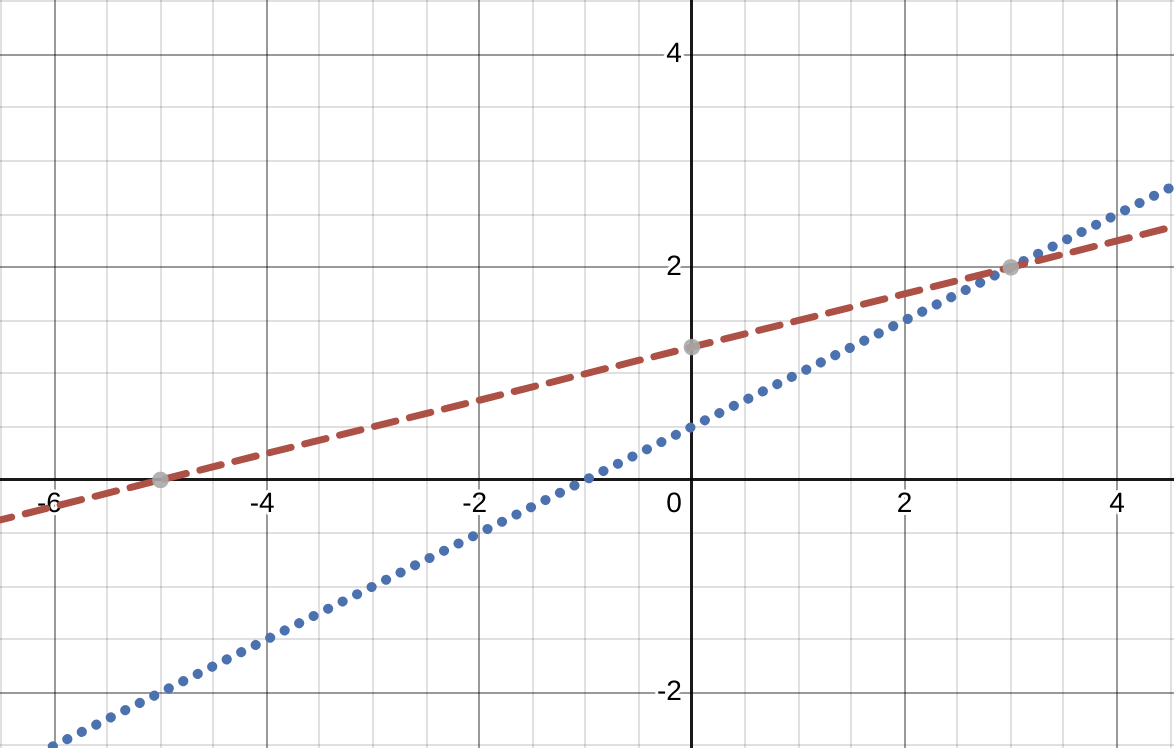
\includegraphics[width=0.9\textwidth]{figures/unique_soln.png}}
        \only<2>{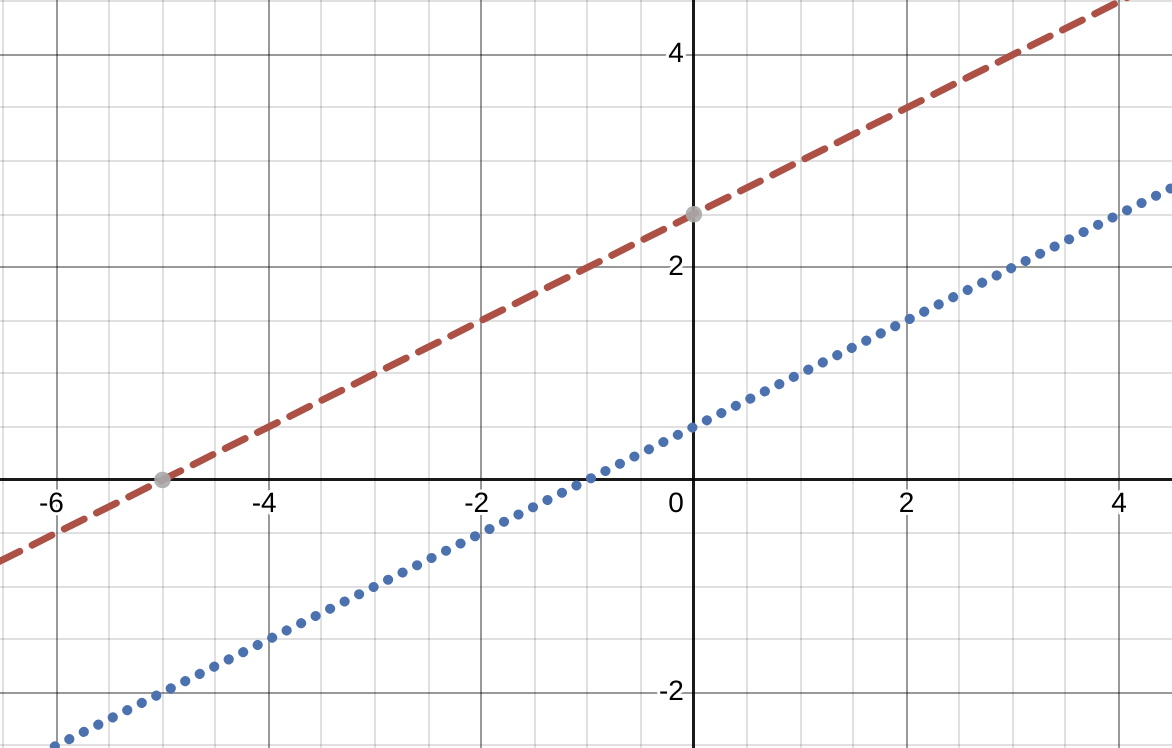
\includegraphics[width=0.9\textwidth]{figures/no_soln.png}}
        \only<3>{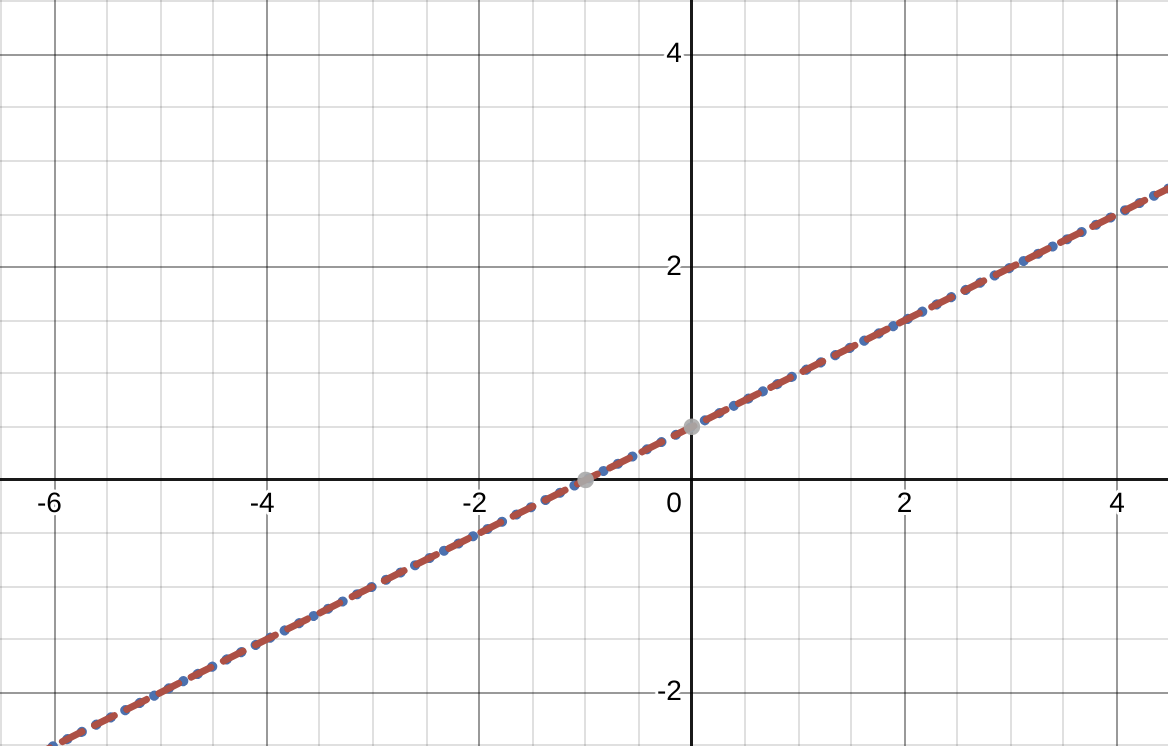
\includegraphics[width=0.9\textwidth]{figures/infinitely_many_soln.png}}
    \end{column}
\end{columns}
    
\end{frame}

\begin{frame}{Solving Systems of Equations}
    \only<1>{
    A linear system may be represented as a matrix and solved using a series of the following row operations:
    \begin{itemize}
        \item \textbf{Replacement}: Replace one row by the sum of itself and a multiple of another row.
        \item \textbf{Interchange}: Interchange two rows.
        \item \textbf{Scaling}: Multiply all entries in a row by a nonzero real number.
    \end{itemize}
    For instance, the linear system
        \begin{align*}
            -2x_1 + 4x_2 + 6x_3 =& 2\\
             -x_1 + 7x_2 + x_3  =& 5\\
             3x_1 - 7x_2 + 2x_3 =& 1
        \end{align*}
        \text{can be written as}
        \[
        \begin{bmatrix}
            -2 & 4 & 6 &| & 2\\
            -1 & 7 & 1 &| & 5\\
             3 &-7 & 2 &| & 1
        \end{bmatrix}
        \]
        }
    \only<2>{
        \text{We then perform the following row operations:}
        \[
        \begin{bmatrix}
            -2 & 4 & 6 &| & 2\\
            -1 & 7 & 1 &| & 5\\
             3 &-7 & 2 &| & 1
        \end{bmatrix}
        -\frac{1}{2}R_1 \rightarrow R_1
        \begin{bmatrix}
             1 & -2 & -3 &| & -1\\
            -1 &  7 &  1 &| &  5\\
             3 & -7 &  2 &| &  1
        \end{bmatrix}
        \]
        
        \[
         R_1 + R_2 \rightarrow R_2
        \begin{bmatrix}
            1 & -2 & -3 &| & -1\\
            0 &  5 & -2 &| &  4\\
            3 & -7 &  2 &| &  1
        \end{bmatrix}
        -3R_1 + R_3 \rightarrow R_3
        \begin{bmatrix}
            1 & -2 & -3 &| & -1\\
            0 &  5 & -2 &| &  4\\
            0 & -1 & 11 &| &  4
        \end{bmatrix}
        \]
        }
    Complete this row operation so that you have an upper triangular matrix (all values below the main diagonal are zeros) as your \textbf{practice}.
\end{frame}

\begin{frame}{Homework 1}
    \only<1>{
    \textbf{Question Q1} 
    Given the linear system
    \begin{align*}
        x_1 - 2x_2 + x_3 =& 0\\
           2x_2 - 8x_3  =& 8\\
         -4x_1 + 5x_2 + 9x_3 =& -9
    \end{align*}
    \begin{enumerate}[a]
        \item Rewrite the system in matrix notation.
        \item Using elementary row operations only, reduce the system to an upper triangular matrix.
        \item Using the upper triangular matrix, solve for \(x_1,\; x_2,\) and \(x_3\).
        
        \textbf{Note:} \emph{for an inconsistent system, you will not be able to solve the system}
        
        \item Is the system consistent?
    \end{enumerate}
    }

    \only<2>{
    \textbf{Question Q2}
    Given the linear system
        \begin{align*}
            x_2 - 4x_3 =& 8\\
               2x_1 - 3x_2 + 2x_3  =& 1\\
             5x_1 - 8x_2 + 7x_3 =& 1
        \end{align*}
    \begin{enumerate}[a]
        \item Rewrite the system in matrix notation.
        \item Using elementary row operations only, reduce the system to an upper triangular matrix.
        
        \textbf{Hint:} \emph{You may need to swap rows to achieve this.}
        
        \item Using the upper triangular matrix, solve for \(x_1,\; x_2,\) and \(x_3\).
        \textbf{Note:} \emph{for an inconsistent system, you will not be able to solve the system.}
        
        \item Is the system consistent?
    \end{enumerate}
    }
\end{frame}


\begin{frame}{Row Reduction and Echelon Forms}
    A rectangular matrix is in \textbf{echelon form} if it has the following properties:
    \begin{columns}
    \begin{column}{0.5\textwidth}
    \begin{itemize}
        \item Any row with all zeros should be moved to the last row.
        \only<1>{\item Each leading entry should have only zeros below it in that column.}
        \only<2>{\item Each leading entry should be \(\mathbf{1}\) and have only zeros below and above it in that column.}
    \end{itemize}
    \textbf{Note:} a leading entry is the first nonzero term in a row.
    \end{column}

    \begin{column}{0.5\textwidth}
        \only<1>{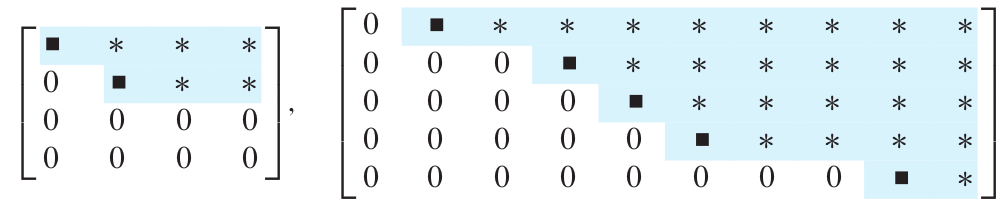
\includegraphics[width=0.9\textwidth]{figures/row_ech.png}}
        \only<2>{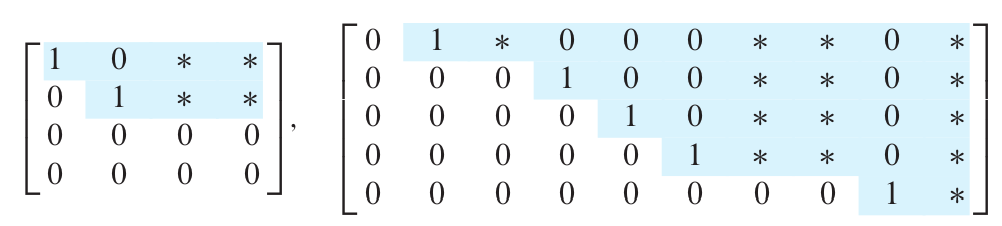
\includegraphics[width=0.9\textwidth]{figures/reduced_row_ech.png}}
    \end{column}
    \end{columns}
    \begin{theorem}[Uniqueness of the Reduced Echelon Form]
        Each matrix is equivalent to one and only one reduced echelon matrix.
    \end{theorem}
    
\end{frame}



\begin{frame}{Example}
Row reduce the matrix below to \textbf{reduced} echelon form
\[
A = \begin{bmatrix} 
0 & -3 & -6 & 4 & 9 \\
-1 & -2 & -1 & 3 & 1 \\
-2 & -3 & 0 & 3 & -1 \\
1 & 4 & 5 & -9 & -7
\end{bmatrix}.
\]
Echelon form:
\[
A = \begin{bmatrix} 
1 & 4 & 5 & -9 & -7 \\
0 & 2 & 4 & -6 & -6 \\
0 & 0 & 0 & -5 &  0 \\
0 & 0 & 0 &  0 &  0
\end{bmatrix}.
\]    
\end{frame}


\begin{frame}{Solving Linear Systems with Row Reductions}
    Suppose your row reduction yields the following, we solve using back substitution;
    \[
    \begin{bmatrix}
            1 & -2 & -3 &| & -1\\
            0 &  1 & -2 &| &  4\\
            0 &  0 &  0 &| &  0
        \end{bmatrix}.
    \]
    We say that \(x_3\) is a free variable, and hence
    \begin{align*}
        x_3=&x_3,\\
            & \\
        x_2 - 2x_3 =& 4\\
        \text{so, } x_2 =& 4 + 2x_3 \text{, and }\\
            & \\
        x_1 - 2x_2 - 3x_3 =& -1\\
        \text{so, } x_1 =& -1 + 2x_2 + 3x_3.\\
        \text{Thus, }  x_1 =& -1 + 2(4 + 2x_3) + 3x_3\\
        =& 7 + 7x_3.
    \end{align*}

\end{frame}


\begin{frame}{Homework 2}
    Determine whether each of the following matrices is in \textit{echelon form}, \textit{reduced echelon form}, or \textit{neither}. Justify your answers.

\textbf{Given Matrices:}
\[
A_1 = \begin{bmatrix} 
1 & 2 & 3 \\
0 & 4 & 5 \\
0 & 0 & 6 
\end{bmatrix}, \quad
A_2 = \begin{bmatrix} 
1 & 0 & 0 \\
0 & 1 & 0 \\
0 & 0 & 1 
\end{bmatrix}, \quad
A_3 = \begin{bmatrix} 
1 & 2 & 3 \\
0 & 1 & 0 \\
0 & 0 & 0 
\end{bmatrix},
\]
\[
A_4 = \begin{bmatrix} 
1 & 2 & 0 \\
0 & 1 & 4 \\
0 & 0 & 1 
\end{bmatrix}, \quad
A_5 = \begin{bmatrix} 
0 & 1 & 2 \\
1 & 0 & 3 \\
0 & 0 & 4 
\end{bmatrix}, \quad
A_6 = \begin{bmatrix} 
1 & 2 & 3 \\
0 & 1 & 0 \\
0 & 0 & 1 
\end{bmatrix}.
\]
\end{frame}



%===================================================================
\subsection{Vector and Matrix Equations}
%===================================================================
\begin{frame}{Vectors}
Linear algebra is a branch of mathematics that focuses on the study of \textbf{vectors}, the space within which they exist (\textbf{vector spaces}) as well as their characteristics and operations that can be performed on them.
Provides a mathematical framework for analyzing systems of linear equations and their representations in higher dimensions.

\begin{columns}
    \begin{column}{0.6\textwidth}
    % \only<1>%{\begin{figure}
    % \begin{tikzpicture}
    %   % Draw vector 1
    %   \draw[->, thick] (-1,1) -- (1,3) node[anchor=south west];
    %   \node at (-0.5, 1.5) [anchor=east] {$\textbf{b}$};
    %   % Draw vector 2
    %   \draw[->, thick] (-1,-.5) -- (1,1.5) node[anchor=south west];
    %   \node at (0, 1) [anchor=west] {$\textbf{b}$};
    %   % Draw vector 3
    %   \draw[->, thick] (1,-.5) -- (4,2.5) node[anchor=south west];
    %   \node at (2, 1) [anchor=west] {$\textbf{a}$};
    %   % Draw vector 4
    %   \draw[<-, thick] (1,2) -- (3,3) node[anchor=south west];
    %   \node at (1.7, 2.3) [anchor=west]{$\textbf{c}$};
    % \end{tikzpicture}
    %\end{figure}}
    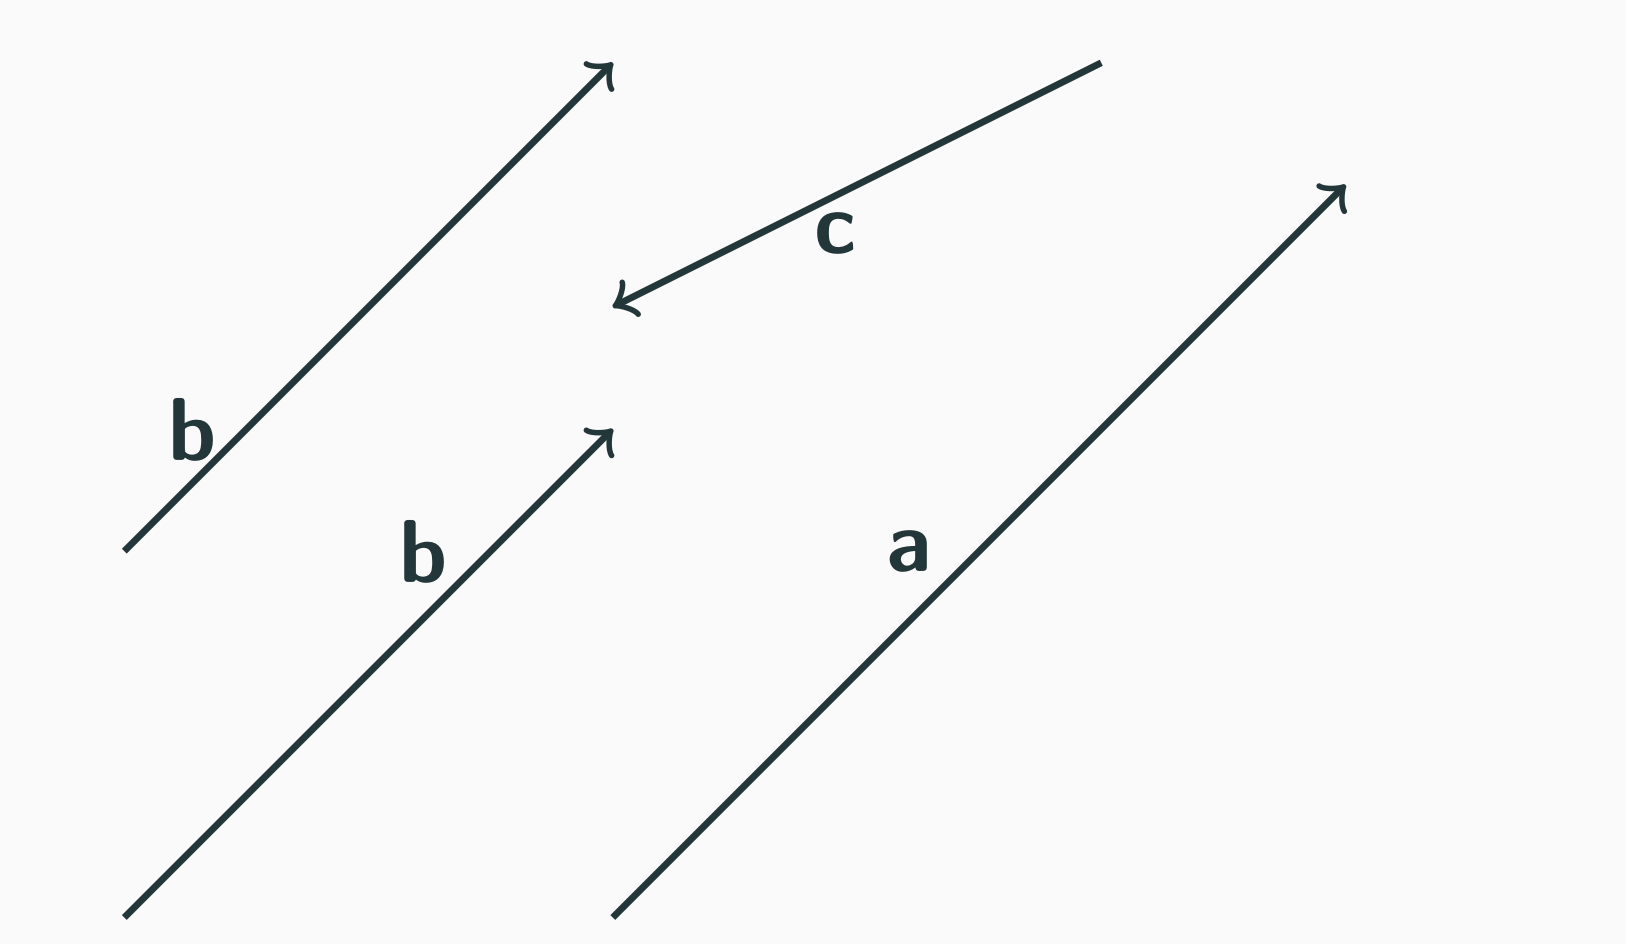
\includegraphics[width=\textwidth]{figures/vectors.png}
    Vectors have \textbf{magnitude} and \textbf{direction} (arrows pointing in space)
    
    \end{column}
    
    % Second column: Text
    \begin{column}{0.4\textwidth}
        Another View is that Vectors are \textbf{ordered lists of numbers}.
        Consider the model for the price of gold.
        \[
        \begin{bmatrix}
            1\text{oz}\\
            \$ 1200
        \end{bmatrix}
        \neq 
        \begin{bmatrix}
            \$1200\\
            1\text{oz}
        \end{bmatrix}
        \]
    \end{column}
\end{columns}
\end{frame}



\begin{frame}{Vectors}
\begin{columns}
    \begin{column}{0.4\textwidth}
    \only<1>{\begin{figure}
        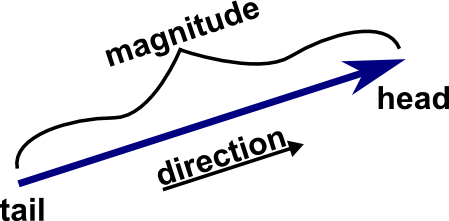
\includegraphics[width=0.9\textwidth]{figures/vector.png}
        \caption{\tiny{\url{https://mathinsight.org/vector_introduction}}}
    \end{figure}}
    
    \only<2>{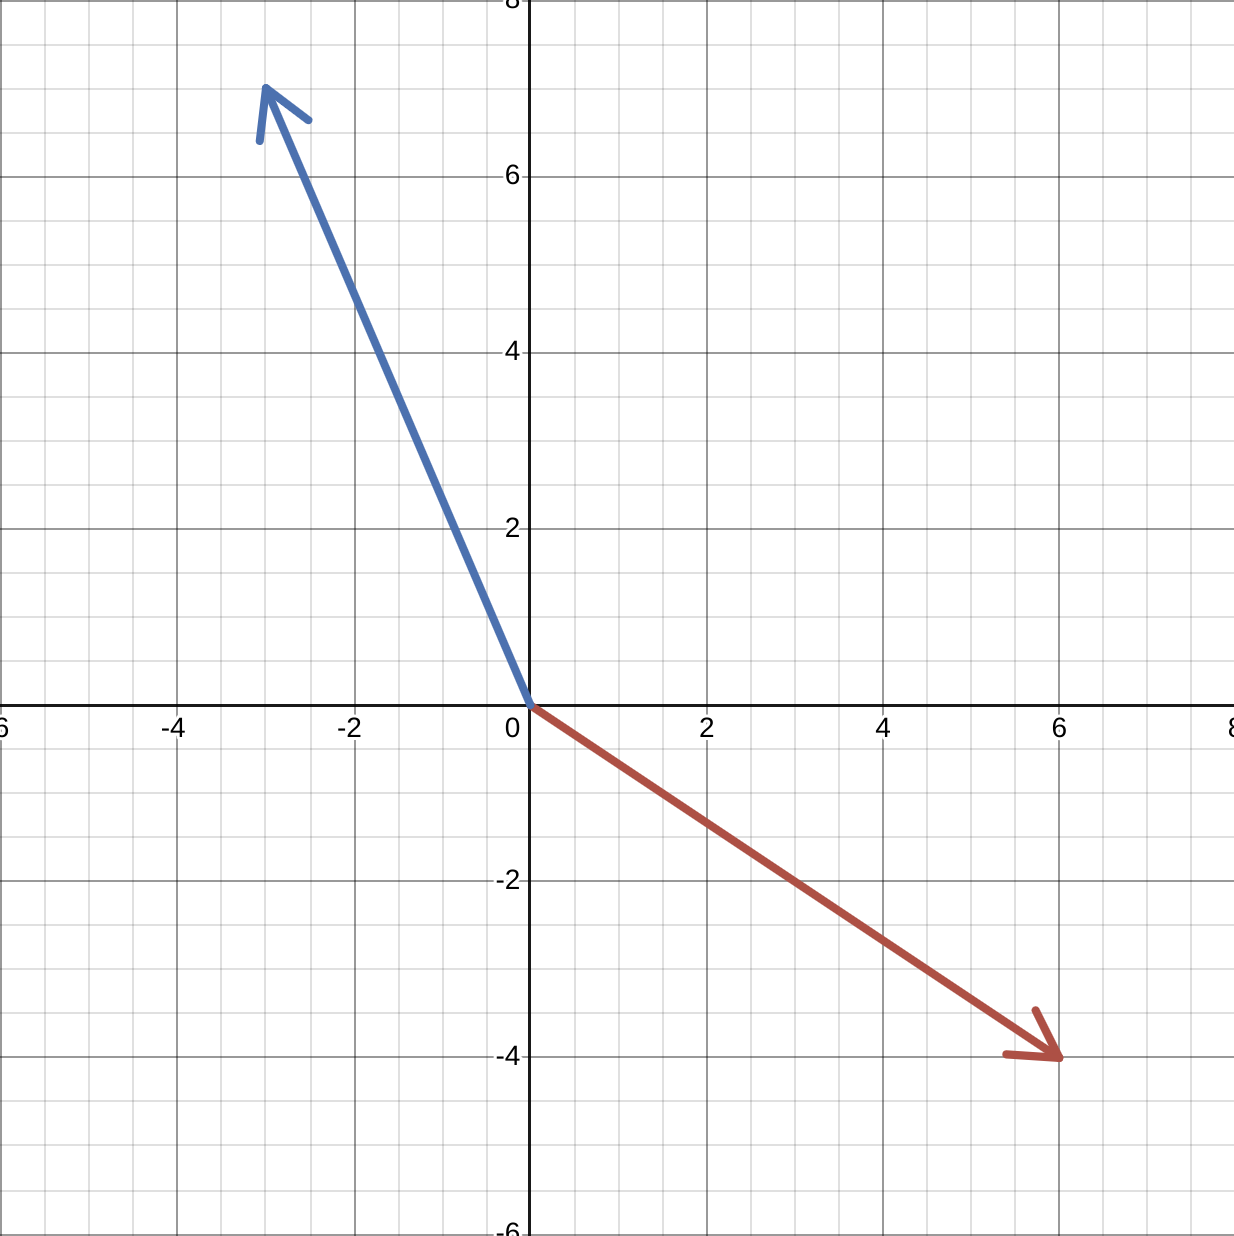
\includegraphics[width=\textwidth]{figures/Two_dimensional_vectora.png}
    \[
    \text{Consider the vectors}
    \begin{bmatrix}
        -3\\7
    \end{bmatrix}
    \text{ and }
    \begin{bmatrix}
        6\\
        -4
    \end{bmatrix}
    \]
    }
    
    \only<3>{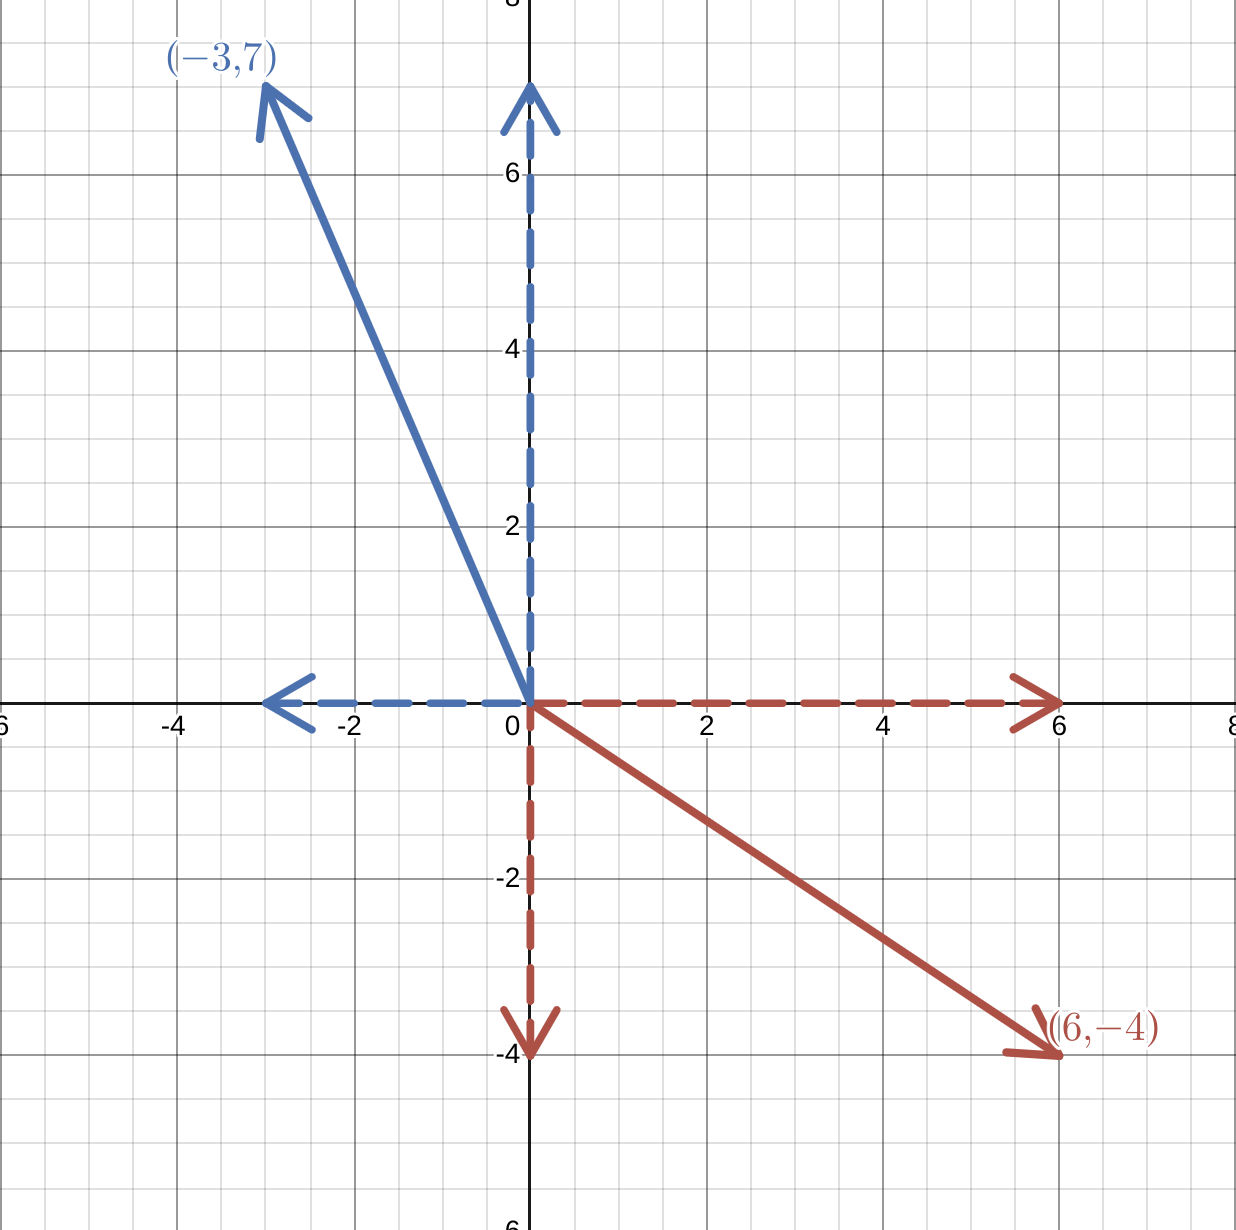
\includegraphics[width=\textwidth]{figures/Two_dimensional_vectorb.png}
    \[
    \text{Consider the vectors}
    \begin{bmatrix}
        -3\\7
    \end{bmatrix}
    \text{ and }
    \begin{bmatrix}
        6\\
        -4
    \end{bmatrix}
    \]
    }
    \end{column}
    % Second column: Text
    \begin{column}{0.6\textwidth}
        \only<1>{In this course when we say vectors we will be referring to a directed line segment sitting at the origin.}
        \begin{itemize}
            \only<1>{\item The two numbers (coordinates) are a pair of numbers that tell you how to get from the tail(origin) to the head(tip)}
            \only<2>{\item The first number tells you how far to walk on the \(x-\)axis. \textbf{Positive} numbers mean \textbf{right}, and \textbf{negative} numbers mean \textbf{left}.}
            \only<2>{\item The second number tells you how far to walk parallel to the \(y-\)axis. \textbf{Positive} numbers mean \textbf{up}, and \textbf{negative} numbers mean \textbf{down}.}
            \only<2>{\item Every pair of numbers is associated with only one vector (arrow), and every vector (arrow) is associated with only one pair of numbers.}
            % this is a repetition for <only 3>
            \only<3>{\item The first number tells you how far to walk on the \(x-\)axis. \textbf{Positive} numbers mean \textbf{right}, and \textbf{negative} numbers mean \textbf{left}.}
            \only<3>{\item The second number tells you how far to walk parallel to the \(y-\)axis. \textbf{Positive} numbers mean \textbf{up}, and \textbf{negative} numbers mean \textbf{down}.}
            \only<3>{\item Every pair of numbers is associated with only one vector (arrow), and every vector (arrow) is associated with only one pair of numbers.}
        \end{itemize}
    \end{column}
\end{columns}
\end{frame}



\begin{frame}{Addition of Vectors and Scalar Multiplication}
\begin{columns}
    \begin{column}{0.5\textwidth}
        Since vectors are ordered (component-wise), addition is also component-wise.
        \begin{itemize}
            \only<1>{\item \textbf{Addition}: Subtraction is also a form of addition
            \[
            \begin{bmatrix}
                -3\\7
            \end{bmatrix}
            +
            \begin{bmatrix}
                6\\
                -4
            \end{bmatrix}
            =
            \begin{bmatrix}
                3\\3
            \end{bmatrix}
            \]
            }
            \only<2>{\item \textbf{Scalar Multiplication}
            \[
            -v_1=
            -
            \begin{bmatrix}
                3\\
                6
            \end{bmatrix}
            =
            \begin{bmatrix}
                -3\\-6
            \end{bmatrix}
            \]
            }
            \only<3>{\item \textbf{Scalar Multiplication}
            \[
            3v_2=
            3
            \begin{bmatrix}
                2\\
                3
            \end{bmatrix}
            =
            \begin{bmatrix}
                6\\9
            \end{bmatrix}
            \]
            }
        \end{itemize}

    \only<3>{
    Note: a vector can have more than 2 dimensions.
    \[
    \begin{bmatrix}
        2\\3\\5
    \end{bmatrix} \text{ is a 3-dimensional vector, and}
    \begin{bmatrix}
        x_1\\ \vdots \\ x_n
    \end{bmatrix} \text{ is n-dimensional vector.}
    \]
    }
    \end{column}
    
    % Second column: Text
    \begin{column}{0.35\textwidth}
    \only<1>{\begin{figure}
        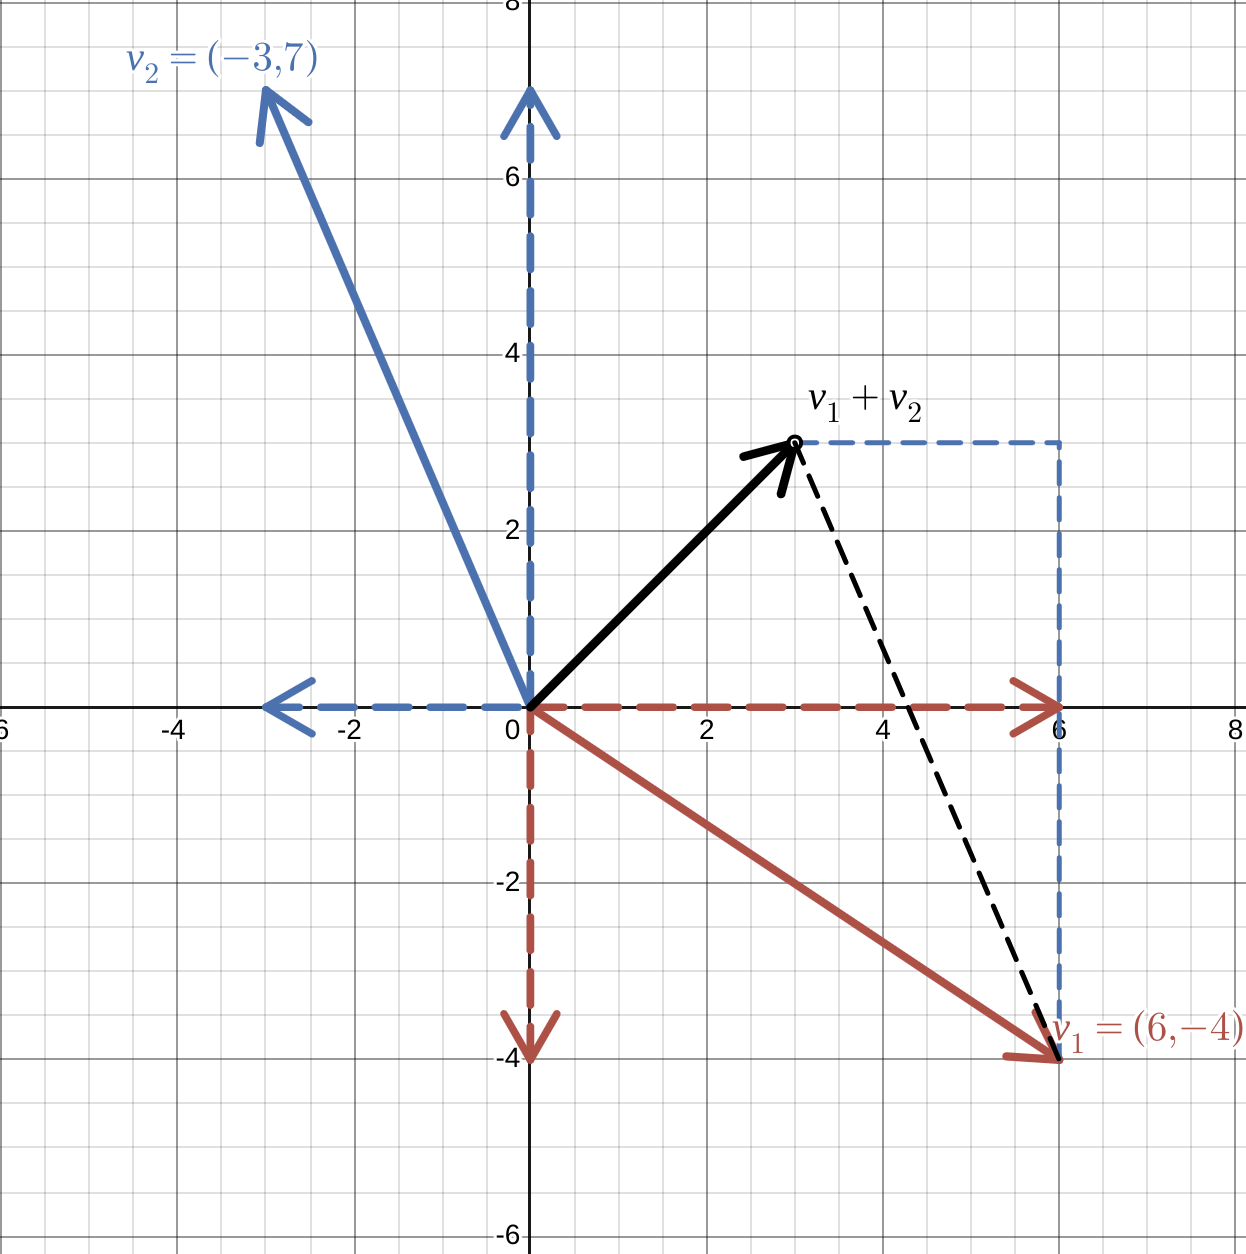
\includegraphics[width=\textwidth]{figures/Two_dimensional_vector_addition.png}
        \caption{Vector Addition}
    \end{figure}}
    \only<2>{\begin{figure}
        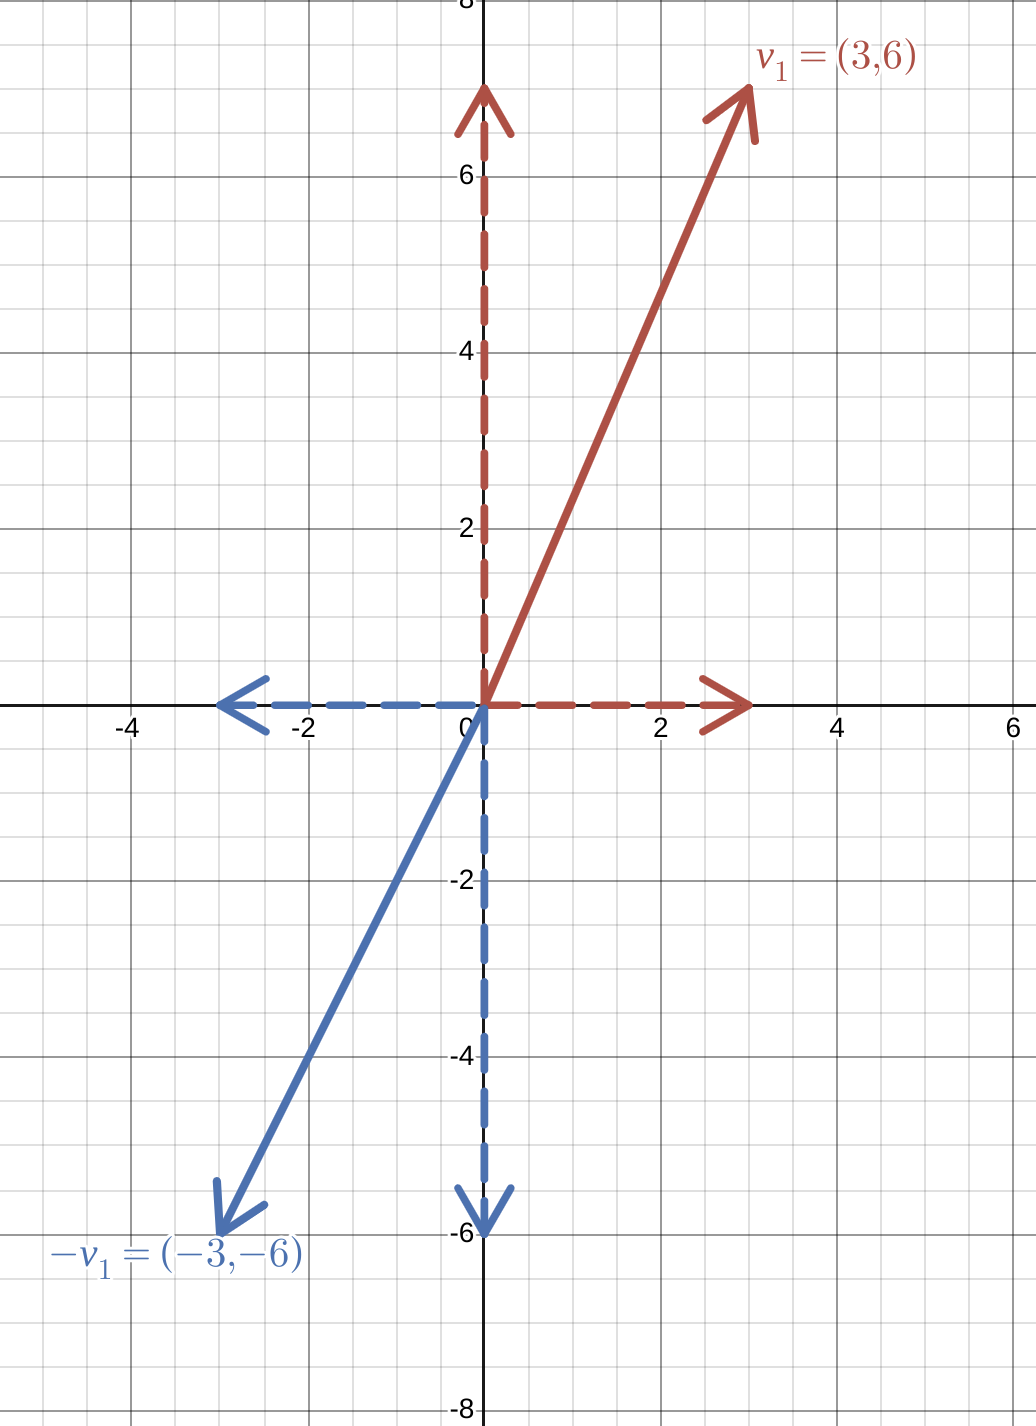
\includegraphics[height=0.8\textheight, width=0.9\textwidth]{figures/Two_dimensional_scalar_multiplication_a.png}
        \caption{Scalar Multiplication}
    \end{figure}}
    \only<3>{\begin{figure}
        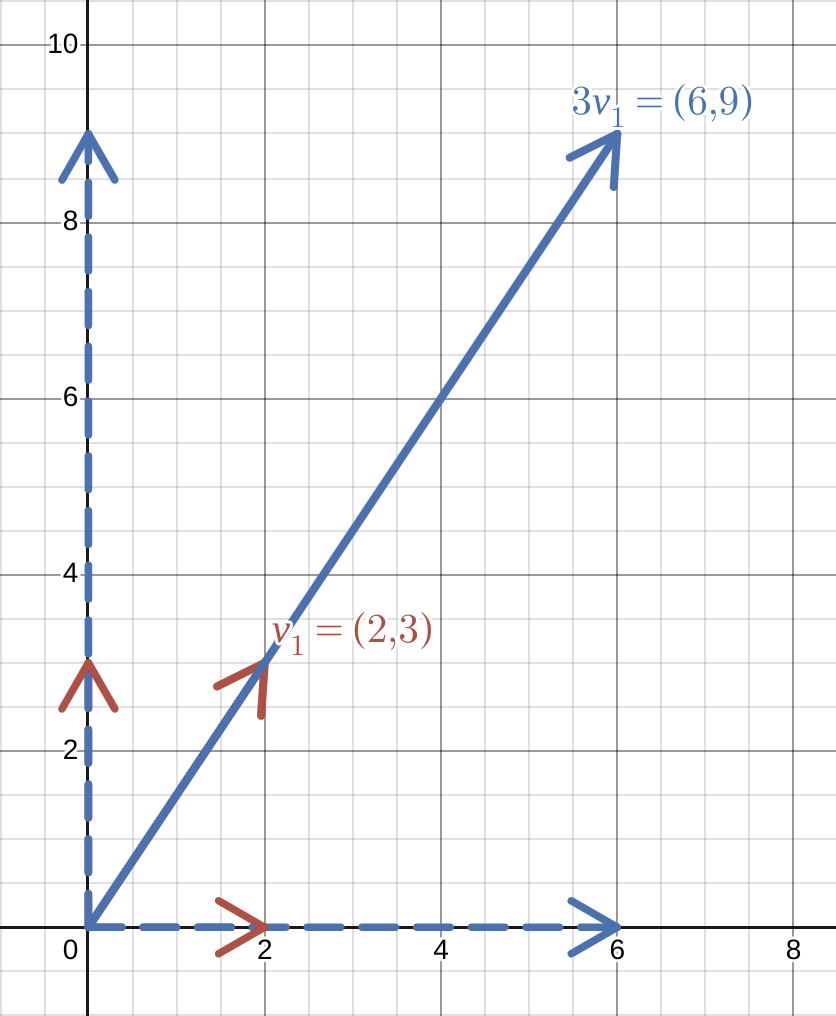
\includegraphics[height=0.7\textheight, width=0.9\textwidth]{figures/Two_dimensional_scalar_multiplication_b.png}
        \caption{Scalar Multiplication}
    \end{figure}}
    \end{column}
\end{columns}
\end{frame}
%================================================================================



\begin{frame}{Special Vectors (Basis)}
\begin{columns}
    \begin{column}{0.6\textwidth}
        Consider the special vectors 
        \(\mathbf{\hat{i}} = \begin{bmatrix}
                1\\0
            \end{bmatrix}\)
        and 
        \(\mathbf{\hat{j}} = \begin{bmatrix}
                0\\1
            \end{bmatrix}\).
        Observe that the vectors 
        \(\begin{bmatrix}
                -3\\7
            \end{bmatrix}
            \text{ and }
            \begin{bmatrix}
                6\\
                -4
            \end{bmatrix}
        \)
        can be written as a sum and scalar multiplication of \(\mathbf{\hat{i}}\) and \(\mathbf{\hat{j}}\).
        \(
            \begin{bmatrix}
                -3\\7
            \end{bmatrix}
            = -3\mathbf{\hat{i}} + 7\mathbf{\hat{j}},
        \) 
        and
        \(
            \begin{bmatrix}
                6\\
                -4
            \end{bmatrix}
            = \; 6\mathbf{\hat{i}} - 4\mathbf{\hat{j}}
        \).
        
        \vspace{0.2cm}
        
        All the vectors you can reach using only vector addition and scalar multiplication is called the \textbf{span} of these special vectors \(\mathbf{\hat{i}}\) and \(\mathbf{\hat{j}}\).
        This is also known as the \textbf{line}ar combination of  \(\mathbf{\hat{i}}\) and \(\mathbf{\hat{j}}\) (Desmos illustration \url{https://www.desmos.com/calculator/apimvn3ln9})
    \end{column}
    
    % Second column: Text
    \begin{column}{0.4\textwidth}
    \only<1>{\begin{figure}
        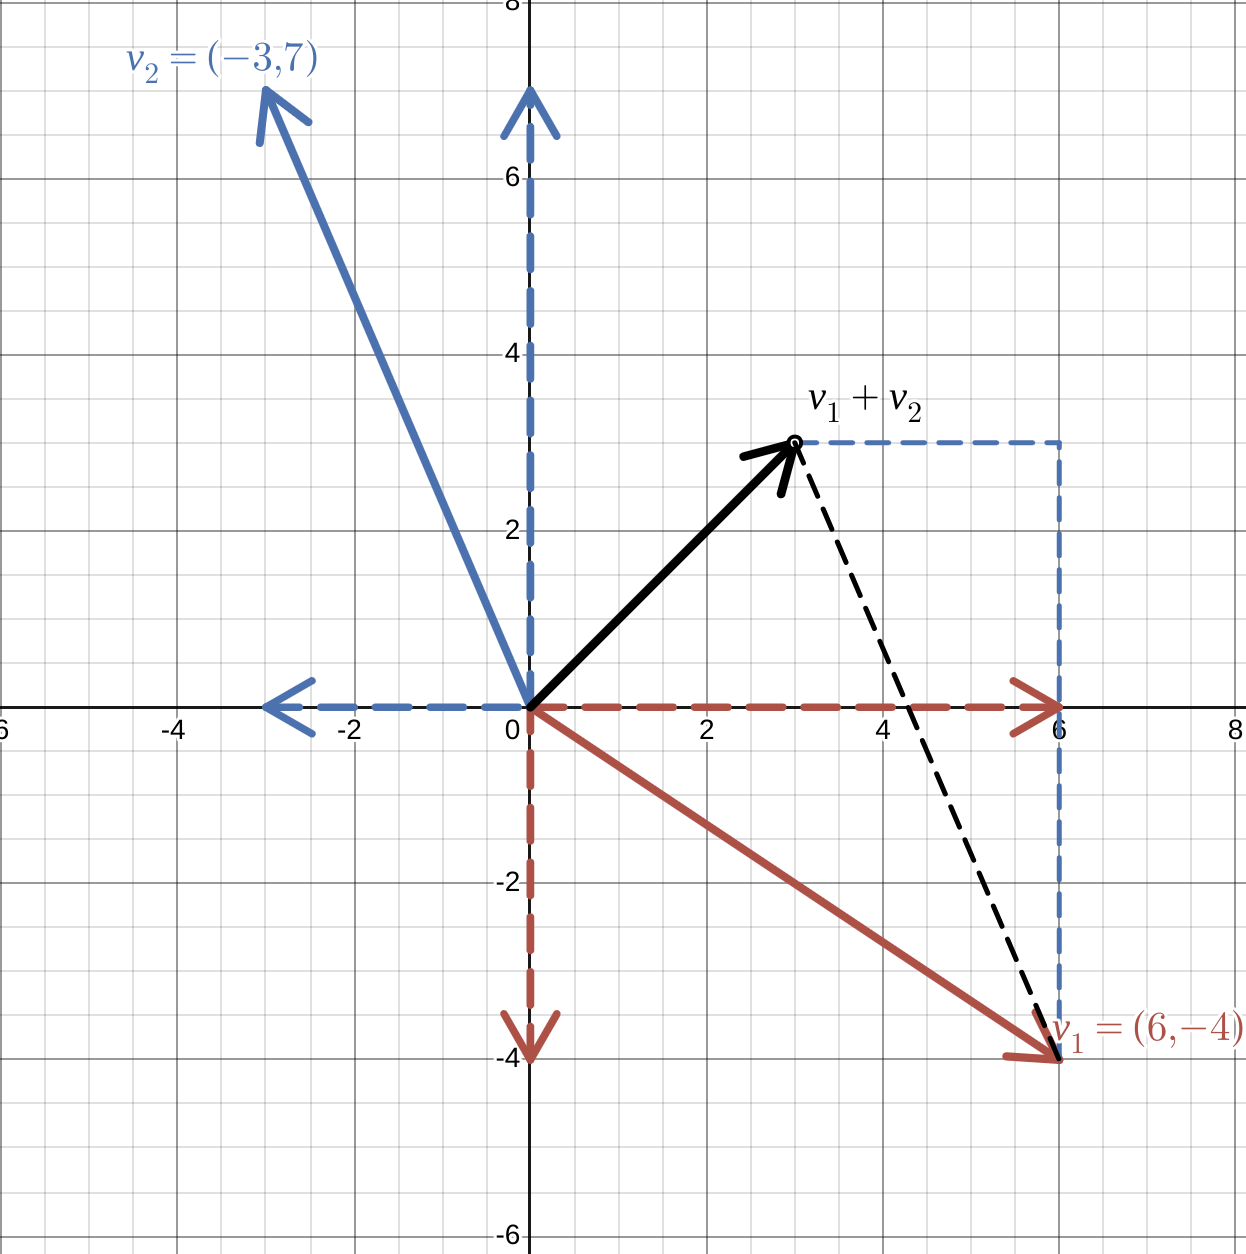
\includegraphics[width=\textwidth]{figures/Two_dimensional_vector_addition.png}
        \caption{Vector Addition}
    \end{figure}}
    \end{column}
\end{columns}
\end{frame}



\begin{frame}{Algebraic Properties of Vectors in \(\mathbb{R}^n\) and Matrix Equations}
    \begin{columns}
    \begin{column}{0.4\textwidth}
    
    \begin{itemize}
        \item \textbf{Commutative Property:} \( \mathbf{u} + \mathbf{v} = \mathbf{v} + \mathbf{u} \)
        \item \textbf{Associative Property:} \( (\mathbf{u} + \mathbf{v}) + \mathbf{w} = \mathbf{u} + (\mathbf{v} + \mathbf{w}) \)
        \item \textbf{Additive Identity:} \( \mathbf{u} + \mathbf{0} = \mathbf{u} \)
        \item \textbf{Additive Inverse:} \( \mathbf{u} + (-\mathbf{u}) = \mathbf{0} \)
        \item \textbf{Distributive Property:} \( r(\mathbf{u} + \mathbf{v}) = r\mathbf{u} + r\mathbf{v} \)
    \end{itemize}

    \scriptsize{
    Where \(\mathbf{u}\), \(\mathbf{v}\), and \(\mathbf{w}\) are vectors.
    \(r\) is a scalar 
    \vspace{0.2cm}
    }
    \end{column}
    
    
    % Second column: Text
    \begin{column}{0.6\textwidth}
    A vector equation \[x_1\mathbf{v_1} + x_2\mathbf{v_2} + \cdots + x_n\mathbf{v_n} = \mathbf{w}\]
    has the same solution set as the linear system whose augmented matrix is
    \[
    \begin{bmatrix}
        \mathbf{v_1} \; \mathbf{v_2} \; \cdots \; \mathbf{v_n} \;  \mathbf{w}
    \end{bmatrix}.
    \]

    In the vector equation, we say that \(\mathbf{w}\) is a linear combination of  \(\mathbf{v_1}, \, \mathbf{v_2}, \, \cdots, \, \mathbf{v_n}. \)

    \end{column}
    \end{columns}

    \begin{definition}[\(Span\) of a Set of Vectors]
        The \(span\) of a set of vectors \(\mathbf{v_1}, \, \mathbf{v_2}, \, \cdots, \, \mathbf{v_p} \in \mathbb{R}^n\) is the set of all possible linear combinations of  \(\mathbf{v_1}, \, \mathbf{v_2}, \, \cdots, \, \mathbf{v_p}\).
    \end{definition}
    That is, if a vector \(\mathbf{b}\) is in \(Span\{\mathbf{v_1}, \, \mathbf{v_2}, \, \cdots, \, \mathbf{v_p}\}\), then \(\mathbf{b} = c_1\mathbf{v_1} + c_2\mathbf{v_2} + \cdots + c_p\mathbf{v_p}\).
\end{frame}



\begin{frame}{Matrix Multiplication}

\only<1>{
Here are some examples to illustrate multiplication of matrices and vectors with different dimensions, showcasing various matrix equations: 

\textbf{Example 1}: Multiplication of a Matrix and a Column Vector

\[
A = 
\begin{bmatrix}
2 & 3 \\
4 & 1 \\
\end{bmatrix}, \quad
\mathbf{v} = 
\begin{bmatrix}
5 \\
6
\end{bmatrix}
\]}

\only<2>{Matrix dimensions: \( A \) (2×2), \( \mathbf{v} \) (2×1)

The product is:
\[
A \mathbf{v} =
\begin{bmatrix}
\mathcolor{red}{2} & \mathcolor{red}{3} \\
4 & 1
\end{bmatrix}
\begin{bmatrix}
\mathcolor{blue}{5} \\
\mathcolor{blue}{6}
\end{bmatrix}
=
\begin{bmatrix}
\mathcolor{red}{2} \cdot \mathcolor{blue}{5} + \mathcolor{red}{3} \cdot \mathcolor{blue}{6} \\
4 \cdot 5 + 1 \cdot 6
\end{bmatrix}
=
\begin{bmatrix}
28 \\
26
\end{bmatrix}
\]}



\only<3>{\textbf{Example 2}: Multiplication of Two Matrices**
\[
B = 
\begin{bmatrix}
1 & 2 & 3 \\
4 & 5 & 6
\end{bmatrix}, \quad
C = 
\begin{bmatrix}
7 & 8 \\
9 & 10 \\
11 & 12
\end{bmatrix}
\]}

\only<4>{Matrix dimensions: \( B \) (2×3), \( C \) (3×2)
The product is:
\[
BC =
\begin{bmatrix}
\mathcolor{red}{1} & \mathcolor{red}{2} & \mathcolor{red}{3} \\
4 & 5 & 6
\end{bmatrix}
\begin{bmatrix}
\mathcolor{blue}{7} & \mathcolor{cyan}{8} \\
\mathcolor{blue}{9} & \mathcolor{cyan}{10} \\
\mathcolor{blue}{11} & \mathcolor{cyan}{12}
\end{bmatrix}
=
\begin{bmatrix}
\mathcolor{red}{1} \cdot \mathcolor{blue}{7} + \mathcolor{red}{2} \cdot \mathcolor{blue}{9} + \mathcolor{red}{3} \cdot \mathcolor{blue}{11} & \mathcolor{red}{1} \cdot \mathcolor{cyan}{8} + \mathcolor{red}{2} \cdot \mathcolor{cyan}{10} + \mathcolor{red}{3} \cdot \mathcolor{cyan}{12} \\
4 \cdot 7 + 5 \cdot 9 + 6 \cdot 11 & 4 \cdot 8 + 5 \cdot 10 + 6 \cdot 12
\end{bmatrix}
=
\begin{bmatrix}
58 & 64 \\
139 & 154
\end{bmatrix}
\]}

\only<5>{ \textbf{Example 3}: Multiplication Involving a Row Vector and a Matrix
\[
\mathbf{u} = 
\begin{bmatrix}
1 & 2 & 3
\end{bmatrix}, \quad
D = 
\begin{bmatrix}
4 & 5 \\
6 & 7 \\
8 & 9
\end{bmatrix}
\]}

\only<6>{\textbf{Matrix dimensions:} \( \mathbf{u} \) (1×3), \( D \) (3×2)
The product is:
\[
\mathbf{u}D =
\begin{bmatrix}
1 & 2 & 3
\end{bmatrix}
\begin{bmatrix}
4 & 5 \\
6 & 7 \\
8 & 9
\end{bmatrix}
=
\begin{bmatrix}
1 \cdot 4 + 2 \cdot 6 + 3 \cdot 8 & 1 \cdot 5 + 2 \cdot 7 + 3 \cdot 9
\end{bmatrix}
=
\begin{bmatrix}
40 & 46
\end{bmatrix}
\]}

\only<7>{\textbf{Example 4:} Non-Conformable Matrices
\[
E = 
\begin{bmatrix}
1 & 2 & -1 \\
3 & 4 &  0
\end{bmatrix}, \quad
F = 
\begin{bmatrix}
5 & 6 \\
7 & 8
\end{bmatrix}
\]}

\only<8>{Matrix dimensions: \( E \) (2×3), \( F \) (2×2)

You cannot multiply \( EF \) because the number of columns in \( E \) does not match the number of rows in \( F \). However, if their roles are reversed (\( FE \)), multiplication is possible, resulting in another \( 2 \times 3 \) matrix.
}
\end{frame}



\begin{frame}{Matrix Equations}
    Recall: A vector equation 
    \begin{align}\label{vector_eq}
    x_1\mathbf{v_1} + x_2\mathbf{v_2} + \cdots + x_n\mathbf{v_n} = \mathbf{w}.
    \end{align}

   Equation \eqref{vector_eq} may be rewritten (with columns as vectors) as 
   \begin{align*}
       [\mathbf{v_1} \; \mathbf{v_2} \; \cdots \; \mathbf{v_n}]
       \begin{bmatrix}
           x_1\\
           x_2\\
           \vdots\\
           x_n
       \end{bmatrix}
       =& \mathbf{w}
       \\
       \begin{bmatrix}
           v_{11} & v_{12} & \cdots & v_{1n}\\
           v_{21} & v_{22} & \cdots & v_{2n}\\
           \vdots & \vdots & \ddots & \vdots\\
           v_{n1} & v_{n2} & \cdots & v_{nn}
       \end{bmatrix}
       \begin{bmatrix}
           x_1\\
           x_2\\
           \vdots\\
           x_n
       \end{bmatrix}
       =&
       \begin{bmatrix}
           w_1\\
           w_2\\
           \vdots\\
           w_n
       \end{bmatrix}
       \\
       A\mathbf{x} =& \mathbf{w}.
   \end{align*}  
\end{frame}


\begin{frame}{Matrix Equation \(A\mathbf{x}=\mathbf{w}\)}
    \begin{definition}{Matrix Equation}
        If \(A\) is and \(m\times n\) matrix with columns \(\mathbf{v}_1, \mathbf{v}_2,\ldots,\mathbf{v}_n\), and if \(\mathbf{x}\in\mathbb{R}^n\), then the product of $A$ and $\mathbf{x}$, is denoted by \(A\mathbf{x}\), \textcolor{red}{is the linear combination of the columns} of \(A\) using the corresponding entries in \(\mathbf{x}\) as weights; i.e,,

        \[
    A\mathbf{x} = [\mathbf{v_1} \; \mathbf{v_2} \; \cdots \; \mathbf{v_n}]
       \begin{bmatrix}
           x_1\\
           x_2\\
           \vdots\\
           x_n
       \end{bmatrix}
       =
       x_1\mathbf{v_1} + x_2\mathbf{v_2} + \cdots + x_n\mathbf{v_n}
    \]
    \end{definition}
    That is, we view a linear combination of vectors as the product of a matrix and a vector.

    
\end{frame}



\begin{frame}{Formulating Matrix equations}
    For example consider the system of linear equations,
    \begin{align*}
        x_1 + 2x_2 - x_3  =& 4\\
            - 5x_2 + 3x_3 =& 1
    \end{align*}
    The corresponding Matrix equation is
    \begin{align*}
        \begin{bmatrix}
           1 &  2 & -1 \\
           0 & -5 &  3
       \end{bmatrix}
       \begin{bmatrix}
           x_1\\
           x_2\\
           x_3
       \end{bmatrix}
       =
       \begin{bmatrix}
           4\\
           1
       \end{bmatrix}
   \end{align*}
   which is equivalent to the vector equation
   \begin{align*}
       x_1\begin{bmatrix}
           1\\0
       \end{bmatrix}
       +
       x_2\begin{bmatrix}
           2\\-5
       \end{bmatrix}
       +
       x_3\begin{bmatrix}
           -1\\3
       \end{bmatrix}
       =
       \begin{bmatrix}
           4\\1
       \end{bmatrix}.
   \end{align*}
\end{frame}



\begin{frame}{Solution to Matrix Equations}
    \begin{theorem}{Existence of Solutions}
       The equation \(A\mathbf{x}=\mathbf{w}\) has a solution if and only if \(\mathbf{w}\) is a linear combination of the columns of \(A\).
   \end{theorem}
   \vspace{0.2cm}
   
   \textcolor{blue}{How is this related to the \(Span\)?}
   \begin{lemma}
       Let \(A\) be an \(m\times n\) matrix.
       Then the following statements are logically equivalent;
       \begin{itemize}
         \item[(a)] For each \(\mathbf{w} \in \mathbb{R}^m\), the equation \(A\mathbf{x}=\mathbf{w}\) has a solution.
         \item[(b)] Each \(\mathbf{w} \in \mathbb{R}^m\) is a linear combination of the columns of \(A\).
         \item[(c)] The columns of \(A\) span  \(\mathbb{R}^m\).
         \item[(d)] \(A\) has a pivot in every row after row reduction.
       \end{itemize}
   \end{lemma}    
\end{frame}



\begin{frame}{Examples}
    \only<1>{\textbf{Example 1}
    \[
    A=
    \begin{bmatrix}
           1 &  -3 & -4 \\
           -3 & 2 &  6 \\
           5 & -1 &  -8
       \end{bmatrix}
    \]
    \begin{itemize}
        \item Does the equation \(A\mathbf{x} = \mathbf{b} \) have a solution for all possible \(\mathbf{b}\in \mathbb{R}^3\)?
        \item In other words, do the columns of \(A\) span \(\mathbb{R}^3\)?
        \item Alternatively, can any vector, \(\mathbf{b}\in \mathbb{R}^3\) be written as a linear combination of the 3 columns of \(A\)? 
    \end{itemize}

    If it does, write out the form of each \(\mathbf{b}\).
    
    If not, describe the set of all \(\mathbf{b}\) for which \(A\mathbf{x} = \mathbf{b} \) does have a solution.
    }


    \only<2>{
    \textbf{Solution:} according to the lemma in the previous page, each \(A\mathbf{x}=\mathbf{b}\) will have a solution for each \(\mathbf{b}\in\mathbb{R}^3\)  if \(A\) has a pivot in every row. So perform a row reduction to get:
    \[
    \begin{bmatrix}
        1 & -3 & -4 \\
        0 & -7 & -6 \\
        0 & 0 & 0
    \end{bmatrix}.
    \]
    Since row 3 does not have a pivot (no nonzero number in the row), we conclude that \(A\mathbf{x}=\mathbf{b}\) does not have a solution for all \(\mathbf{b}\in\mathbb{R}^3\).
    
    To find the form of \(\mathbf{b}=
    \begin{bmatrix}
        b_1\\
        b_2\\
        b_3
    \end{bmatrix}\), use row reductions with the \(b\)'s in an augmented matrix form.
    \[
        \left[\begin{array}{ccc|c}
               \;\;\;1 &  -3 & -4 & b_1\\
               -3 & \;\;2 &  \;\;6 & b_2\\
               \;\;5 & -1 &  -8 & b_1
        \end{array}\right]
        \begin{array}{c}
             R_2 + 3R_1 \to R_2\\
             R_3 - 5R_1 \to R_3
        \end{array}
        \left[\begin{array}{ccc|c}
            1 & -3 & -4 & b_1\\
            0 & -7 & -6 & b_2 + 3b_1\\
            0 & 14 & 12 & b_3 - 5b_1
        \end{array}\right]
    \]
    }


    \only<3>{
    \[
    \begin{array}{c}
        R_3 + 2R_2 \to R_3
        \end{array}
    \left[\begin{array}{ccc|c}
        1 & -3 & -4 & b_1\\
        0 & -7 & -6 & b_2 + 3b_1\\
        0 & 0 & 0 & 2b_2 + b_1 + b_3 
    \end{array}\right]
    \]
    This matrix equation only has a solution if the entire 3rd row is \(0\). That is, \(2b_2 + b_1 + b_3 =0\) otherwise the system will be inconsistent.
    So, \(b_3 = -b_1 -2b_2\).

    \[
    \text{Thus, } \mathbf{b}
    =
    \begin{bmatrix}
        b_1\\
        b_2\\
        b_3
    \end{bmatrix}
    =
    \begin{bmatrix}
        b_1\\
        b2\\
        -b_1 -2b2
    \end{bmatrix}
    =
    \begin{bmatrix}
        b_1\\
        0\\
        -b_1
    \end{bmatrix}
    +
    \begin{bmatrix}
        0\\
        b_2\\
        2b_2
    \end{bmatrix}
    =
    b_1
    \begin{bmatrix}
        1\\
        0\\
        -1
    \end{bmatrix}
    +
    b_2
    \begin{bmatrix}
        0\\
        1\\
        2
    \end{bmatrix}
    \]
    \[
    \mathbf{b} = 
     \left\{
    b_1
    \begin{bmatrix}
        1\\
        0\\
        -1
    \end{bmatrix}
    +
    b_2
    \begin{bmatrix}
        0\\
        1\\
        2
    \end{bmatrix}, \quad \text{for } b_1,b_2 \in \mathbb{R}
    \right\}.
    \]
    }

    
    \only<4>{\textbf{Example 2}

    Let
    \( \mathbf{v}_1 = 
   \begin{bmatrix}
       \;\;0\\
       \;\;0\\
       -1
   \end{bmatrix} \)
   , 
   \( \mathbf{v}_2 = 
   \begin{bmatrix}
       \;\;0\\
       -3\\
       \;\;2
   \end{bmatrix} \)
   ,
   \( \mathbf{v}_3 = 
   \begin{bmatrix}
       1\\
       3\\
       5
   \end{bmatrix} \).
   Do these 3 vectors span \(\mathbf{R}^3\)?

   \textbf{Solution}: Yes! Reduce to echelon form and observe that each row has a pivot. So, by the previous lemma, the columns span \(\mathbb{R}^3\). 
   }
    

    \only<5>{\textbf{Example 3}

    Let
    \( \mathbf{v}_1 = 
   \begin{bmatrix}
       1\\
       0\\
       -1\\
       0
   \end{bmatrix} \)
   , 
   \( \mathbf{v}_2 = 
   \begin{bmatrix}
       0\\
       -1\\
       0\\
       1
   \end{bmatrix} \)
   ,
   \( \mathbf{v}_3 = 
   \begin{bmatrix}
       1\\
       0\\
       0\\
       -1
   \end{bmatrix} \).
   Do these 3 vectors span \(\mathbf{R}^4\)?

   \textbf{Solution}: No! Reduce to echelon form and observe that the last row has no a pivot. So, by the previous lemma, the columns do not span \(\mathbb{R}^4\). 
   }

   \only<6>{\textbf{Example 4}
   Construct a \(3\times 3\) matrix, \(A\) and vectors \(\mathbf{w},\mathbf{b} \in \mathbb{R}^3\) such that \(A\mathbf{x} = \mathbf{b} \) has a solution, but \(A\mathbf{x} = \mathbf{w}\) does not have a solution.

   \textbf{Solution}: You can use the matrix in example 1. Then choose a vector that meets the condition of \(\mathbf{b}\), and another vector that does not meet that condition. 
   }
\end{frame}


\begin{frame}{Homework3}
\textbf{Question 1}

If \(A\) is an \(3\times 2\) matrix, and \(\mathbf{u}, \;\mathbf{w} \; \in \mathbb{R}^2\) are vectors, show that \(A(\mathbf{u} + c\mathbf{w}) = A\mathbf{u} + cA\mathbf{w}\), where \(c\) is a scalar.

    That is, \(A = [\mathbf{v_1} \; \mathbf{v_2} ]\) and 
    \( \mathbf{u} = 
   \begin{bmatrix}
       u_1\\
       u_2
   \end{bmatrix} \)
   and 
   \( \mathbf{w} = 
   \begin{bmatrix}
       w_1\\
       w_2
   \end{bmatrix} \).


\textbf{Question 2}

Let \(A= 
           \begin{bmatrix}
               2 & -1\\
              -6 &  3 
            \end{bmatrix} \)
and \( \mathbf{b}=
        \begin{bmatrix}
               b_1\\
               b_2
           \end{bmatrix}.
        \)
        
Show that the equation \(A\mathbf{x} = \mathbf{b} \) does not a have a solution for all possible \(\mathbf{b}\), and describe the set of all \(\mathbf{b}\) for which \(A\mathbf{x} = \mathbf{b} \) has a solution.
In other words, do the columns of \(A\) span \(\mathbb{R}^2\)?
\end{frame}



\subsection{Linear Independence and Solution Sets of Linear Systems}
\begin{frame}{Linear Independence and Solution Sets of Linear Systems I}
    \textbf{Recall:} (The \textcolor{blue}{\(Span\)} of a set of vectors \(S=\{\mathbf{v_1}, \; \mathbf{v_2}, \; \mathbf{v_3}\}\), is the set of all the possible linear combinations, \(c_1\mathbf{v_1}, +c_2\mathbf{v_2}+c_3\mathbf{v_3}\)).
    
    Thus, if we can obtain \(\mathbf{v_3}\) by a linear combination of \(\mathbf{v_1}\) and \(\mathbf{v_2},\) then \(\mathbf{v_3}\) is \textcolor{blue}{linearly dependent} on \(\mathbf{v_1}\) and \(\mathbf{v_2}\).
    Otherwise, we say \(\mathbf{v_3}\) is \textcolor{cyan}{linearly independent} of \(\mathbf{v_1}\) and \(\mathbf{v_2}\).

    If linear independence applies for all the elements within the set, we say \(S\) is linearly independent.
    
    \vspace{0.15cm}
    
    \begin{columns}
        \begin{column}{0.5\textwidth}
            \textbf{Example 1} Determine if the following homogeneous system has a nontrivial solution. Then describe the solution set.
            \begin{align*}
                3x_1 + 5x_2 -4x_3 &= 0\\
                -3x_1 - 2x_2 +4x_3 &= 0\\
                6x_1 + \;x_2 -8x_3 &= 0
            \end{align*}
        \end{column}

        \begin{column}{0.5\textwidth}
             Is 
             \(\begin{bmatrix}
                4\\
                0\\
                3
            \end{bmatrix}\) as solution vector?\\
            
            \textbf{Example 2} Determine the solution of the following homogeneous system
            \[10x_1 -3x_2 - 2x_3 = 0.\]
            Write the solution as a parametric vector equation.
        \end{column}
    \end{columns}
    
    \vspace{0.15cm}
    
    A linear system is \textcolor{red}{homogeneous} if it can be written as \(A\mathbf{x}=\mathbf{0}\), where \(A\) is an \(m\times n\) matrix.
\end{frame}

\begin{frame}{Linear Independence and Solution Sets of Linear Systems Part II}
\begin{center}\setlength{\fboxsep}{10pt}\fcolorbox{green!20}{green!20}{\parbox{0.9\linewidth}{
   \begin{theorem}
       Suppose that the equation \(A\mathbf{x}=\mathbf{b}\) is consistent for some given \(\mathbf{b}\), and let \(\mathbf{p}\) be a solution.
       Then the solution set of \(A\mathbf{x}=\mathbf{b}\) is the set of all vectors of the form \(\mathbf{w}=\mathbf{p}+\mathbf{v}_h\), where \(\mathbf{v}_h\) is any solution of the homogeneous solution \(A\mathbf{x}=\mathbf{0}\).
   \end{theorem}
}}
\end{center}

That is, if \(\mathbf{Ax}=\mathbf{b}\) has a solution, then the solution is obtained by translating the solution set of \(\mathbf{Ax}=\mathbf{0}\).

   \textbf{Example 1b} Determine if the following nonhomogeneous system has a nontrivial solution. Then describe the solution set.
        \begin{align*}
            3x_1 + 5x_2 -4x_3 &= 7\\
            -3x_1 - 2x_2 +4x_3 &= -1\\
            6x_1 + x_2 -8x_3 &= -4
        \end{align*}
        
\end{frame}


\begin{frame}{Linear Independence and Solution Sets of Linear Systems Part III}

\begin{center}\setlength{\fboxsep}{10pt}\fcolorbox{black}{blue!20}{\parbox{0.9\linewidth}{
    \begin{definition}[Linear Dependence]
       A set of vectors \( \{ \mathbf{v}_1, \mathbf{v}_2, \dots, \mathbf{v}_n \} \) in a vector space \( V \) is said to be \textcolor{green}{\textit{linearly dependent}} if there exist scalars \( c_1, c_2, \dots, c_n \), not all zero, such that:
    \[
    c_1 \mathbf{v}_1 + c_2 \mathbf{v}_2 + \cdots + c_n \mathbf{v}_n = \mathbf{0}.
    \]
    \end{definition}   

    \begin{definition}[Linear Independence]
        A set of vectors \( \{ \mathbf{v}_1, \mathbf{v}_2, \dots, \mathbf{v}_n \} \) in a vector space \( V \) is said to be \textcolor{magenta}{\textit{linearly independent}} if the only scalars \( c_1, c_2, \dots, c_n \) that satisfy:
    \[
    c_1 \mathbf{v}_1 + c_2 \mathbf{v}_2 + \cdots + c_n \mathbf{v}_n = \mathbf{0}
    \]
are \( c_1 = c_2 = \cdots = c_n = 0 \).
    \end{definition}
}}\end{center}
\end{frame}


\begin{frame}{Linear Independence and Solution Sets of Linear Systems Part IV}
    \begin{lemma}[Linear Independence and Homogeneous Systems]
        The columns of a matrix \(A\) are linearly independent if and only if the homogeneous equation \( A\mathbf{x} = \mathbf{0} \) has only the trivial solution \( \mathbf{x} = \mathbf{0} \).
    \end{lemma}
    \begin{proof}
        \begin{itemize}
            \item \textbf{(\(\Rightarrow\))} Suppose the columns of \( A \) are linearly independent. Then, by definition, the only scalars \( c_1, c_2, \dots, c_n \) that satisfy:
            \[
                c_1 \mathbf{a}_1 + c_2 \mathbf{a}_2 + \cdots + c_n \mathbf{a}_n = \mathbf{0}
            \]
            are \( c_1 = c_2 = \cdots = c_n = 0 \), where \( \mathbf{a}_i \) are the columns of \( A \). This implies that \( A\mathbf{x} = \mathbf{0} \) has only the trivial solution \( \mathbf{x} = \mathbf{0} \).
        
            \item \textbf{(\(\Leftarrow\))} Suppose \( A\mathbf{x} = \mathbf{0} \) has only the trivial solution \( \mathbf{x} = \mathbf{0} \). Then there are no nontrivial combinations of the columns of \( A \) that sum to \( \mathbf{0} \), implying that the columns of \( A \) are linearly independent.
        \end{itemize}
    \end{proof}
\end{frame}

\begin{frame}{Linear Independence and Solution Sets of Linear Systems Part V}
\begin{center}\setlength{\fboxsep}{10pt}\fcolorbox{yellow!20}{yellow!20}{\parbox{0.9\linewidth}{

    \textbf{Example 1}: Determine if the columns of the matrix \( A =\begin{bmatrix}
           0 &  1 & 4 \\
           1 &  2 &-1\\
           5 &  8 & 0
       \end{bmatrix}\) are linearly independent.

    \textbf{Example 2}: Determine if the vectors are \( \begin{bmatrix}
           0\\
           1 \\
           5 
       \end{bmatrix}\), 
       \( \begin{bmatrix}
           -1\\
           2 \\
           5 
       \end{bmatrix}\), 
       \( \begin{bmatrix}
           0\\
           3 \\
           1 
       \end{bmatrix}\) are linearly independent.


    \textbf{Example 3}: Show that the set of two vector \(\{\mathbf{v}_1, \mathbf{v}_2\}\) is linearly dependent if at least one of the vectors is a multiple of the other.
}}
\end{center}

\end{frame}

\begin{frame}{Linear Independence and Solution Sets of Linear Systems Part VI}
\begin{center}\setlength{\fboxsep}{10pt}\fcolorbox{green!20}{green!20}{\parbox{0.9\linewidth}{
    \begin{theorem}{Characterization of Linearly Dependent Sets}
    An indexed set \(S=\{ \mathbf{v}_1, \mathbf{v}_2, \ldots, \mathbf{v}_p \}\) of two or more vectors is linearly dependent if and only if at least one of the vectors in \(S\) is a linear combination of the others.
    That is, each \(\mathbf{v}_i\in S\) does not have to be a linear
    combination of the other vectors.
    Only one of them needs to satisfy the condition.
    \end{theorem}
    }}
\end{center}

\begin{center}\setlength{\fboxsep}{10pt}\fcolorbox{green!20}{green!20}{\parbox{0.9\linewidth}{
\begin{lemma}
    A set \(S=\{ \mathbf{v}_1, \mathbf{v}_2, \ldots, \mathbf{v}_p \} \) whose elements \(\mathbf{v}_i\in\mathbb{R}\) is linearly dependent if $p>n$.
\end{lemma}
}}
\end{center}

\begin{center}\setlength{\fboxsep}{10pt}\fcolorbox{green!20}{green!20}{\parbox{0.9\linewidth}{
\begin{lemma}
    A set \(S=\{ \mathbf{v}_1, \mathbf{v}_2, \ldots, \mathbf{v}_p \} \) whose elements \(\mathbf{v}_i\in\mathbb{R}\) is linearly dependent if one of the elements, \(\mathbf{v}_j=\mathbf{0}\) is the zero vector.
\end{lemma}
}}
\end{center}
\end{frame}


\begin{frame}{Homework 4}
\textbf{Question Q1}

Construct a \(3\times 3\) nonzero matrix such that the vector
    \( \mathbf{u} = 
   \begin{bmatrix}
       1\\
       1\\
       1
   \end{bmatrix} \)
is a solution of \(A\mathbf{x} = \mathbf{b}\).


\textbf{Question Q2}

Are the following vectors linearly dependent? Justify your answer.

\( \mathbf{v_1} = 
   \begin{bmatrix}
       1\\
       1\\
       1
   \end{bmatrix} \), 
   \( \mathbf{v_2} = 
   \begin{bmatrix}
       0\\
       1\\
       3
   \end{bmatrix} \), and 
   \( \mathbf{v_3} = 
   \begin{bmatrix}
       -1\\
       2\\
       1
   \end{bmatrix} \)
\end{frame}



\subsection{Introduction to Linear Transformations}
\begin{frame}{Introduction to Linear Transformations}
A \textcolor{blue}{linear transformation} is a mathematical operation that maps vectors from one vector space to another (or to itself).
This function can be represented as a matrix.

A linear transformation \( T \) from \( \mathbb{R}^n \) to \( \mathbb{R}^m \) can be written as:
\[
T(\mathbf{x}) = A\mathbf{x},
\]
where: \( A \) is an \(m \times n\) matrix (the transformation matrix), \( \mathbf{x} \in \mathbb{R}^n \) is the input vector.
\( T(\mathbf{x}) \in \mathbb{R}^m \) is the transformed vector.

\textbf{Note:} A \textbf{transformation} is just a \textcolor{blue}{function}

A transformation is linear if it has the following properties:
\begin{itemize}
    \item All lines remain lines.
    \item The origin stays the same.
\end{itemize}
\end{frame}


\begin{frame}{Example}
Let \( A=
\begin{bmatrix}
    \;\;1 & -3\\
    \:\:3 & \;\;5\\
    -1 & \;\;7
\end{bmatrix},
\quad
\mathbf{u}=
\begin{bmatrix}
    \;\;2\\-1
\end{bmatrix},
\quad 
\mathbf{b}=
\begin{bmatrix}
    \;\;3 \\ \;\;2 \\ -5
\end{bmatrix},
\quad 
\mathbf{c}=
\begin{bmatrix}
    3 \\ 2 \\ 5
\end{bmatrix},
\)

and define the transformation \( T \;: \;\mathbb{R}^2 \to  \mathbb{R}^3 \) by \(T(\mathbf{x}) = A\mathbf{x}\).
\begin{itemize}
    \item[a.] Find \(T(\mathbf{u})\), the image of \(\mathbf{u}\) under the transformation \(T\).
    \item[b.] Find an \(\mathbf{x}\in\mathbb{R}^2\) such that  \(T(\mathbf{x}) = \mathbf{b}\).
    
    \only<2>{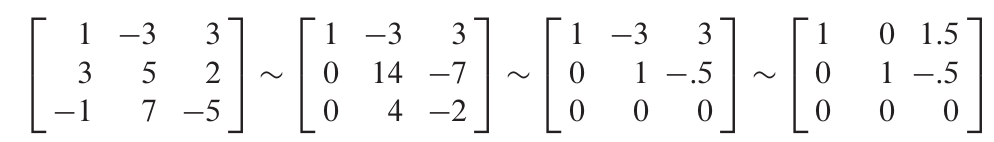
\includegraphics[width=0.7\textwidth]{figures/Solution1.png}}
    \only<3>{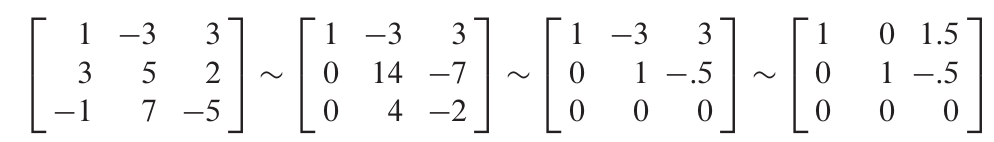
\includegraphics[width=0.7\textwidth]{figures/Solution1.png}}
    
    \item[c.] Is there more than one \(\mathbf{x}\in \mathbb{R}^2\)  such that \(T(\mathbf{x}) = \mathbf{b}\) ?
    \item[d.] Determine if \(\mathbf{c}\) is in the range of the transformation \(T\).
    In other words, is there an \(\mathbf{x}\in\mathbb{R}^2\) such that  \(T(\mathbf{x}) = \mathbf{c}\) ?

    \only<3>{\includegraphics[width=0.7\textwidth]{figures/Solution2.png}}
\end{itemize}
\end{frame}


\begin{frame}{More Examples}
    \textbf{Example 2}: Construct a transformation matrix that projects points in \(\mathbb{R}^3\) to \(\mathbb{R}^2\).

    Can you construct another transformation to do a similar thing?
    \begin{columns}
        \begin{column}{0.7\textwidth}
            \textbf{Example 3}: Let \(A = 
            \begin{bmatrix}
                1 & 3\\
                0 & 1
            \end{bmatrix}.\)
            The transformation \(T:\mathbb{R}^2 \to \mathbb{R}^2\) defined by \(T(\mathbf{x}) = A\mathbf{x}\) is called a \textbf{shear transformation}.

            What does the transformation do to a square?

            \textbf{Hint:} apply the transformation to the points 
            \(
            \left[\begin{array}{c} 0 \\0 \end{array}\right], \; 
            \left[\begin{array}{c} 2 \\0 \end{array}\right], \;
            \left[\begin{array}{c} 0 \\2 \end{array}\right], \; \text{and }
            \left[\begin{array}{c} 2 \\2 \end{array}\right]
            \). These four points form a square of length 2 on each side.

            \only<2>{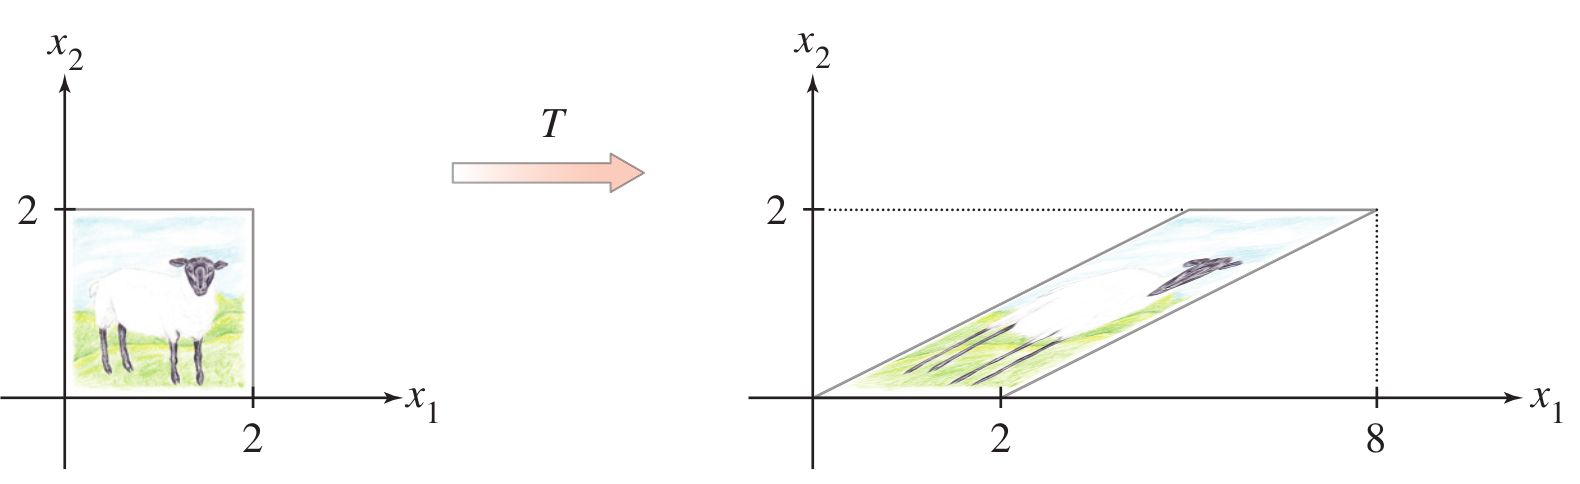
\includegraphics[width=\textwidth]{figures/sheared_sheep.png}}
            \only<3>{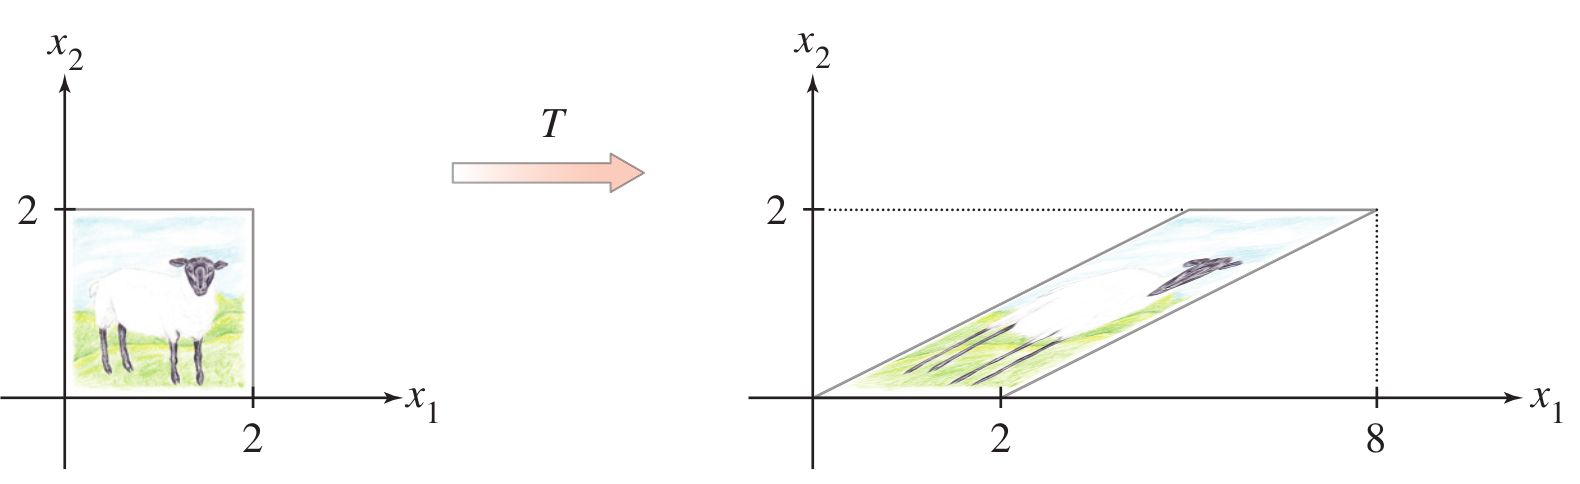
\includegraphics[width=\textwidth]{figures/sheared_sheep.png}}
        \end{column}

        \begin{column}{0.3\textwidth}
            \only<3>{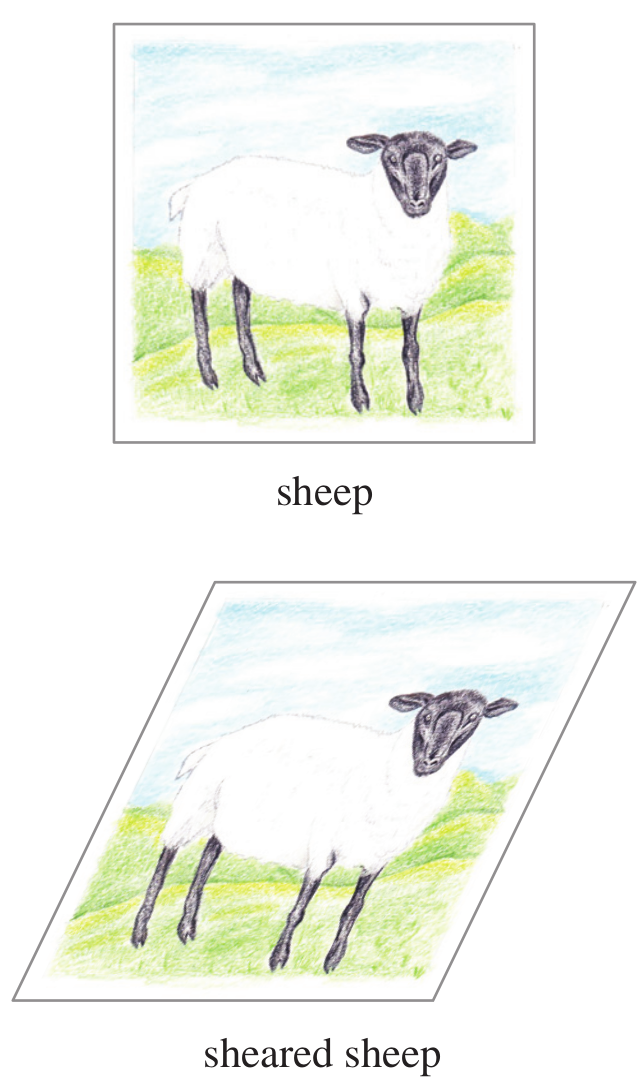
\includegraphics[width=0.9\textwidth]{figures/sheared_sheep_b.png}}
        \end{column}
    \end{columns}

 
\end{frame}


\begin{frame}{Introduction to Linear Transformations}
\begin{center}\setlength{\fboxsep}{10pt}\fcolorbox{blue!20}{blue!20}{\parbox{0.9\linewidth}{
\begin{definition}[Linear Transformation]
    A transformation \( T \) from \( \mathbb{R}^n \) to \( \mathbb{R}^m \) is linear if it satisfies the following:
    
    For any input vector \( \mathbf{u}, \mathbf{v} \in \mathbb{R}^n \) and scalar \(c\in\mathbb{R}\),
    \begin{enumerate}[(i)]
        \item \textbf{Additivity}: \( T(\mathbf{u} + \mathbf{v}) = T(\mathbf{u}) + T(\mathbf{v}) \).
        \item \textbf{Scalar Multiplication}: \( T(c\mathbf{u}) = cT(\mathbf{u}) \), for any scalar \( c \).
    \end{enumerate}
    
\end{definition}
}}
\end{center}

Geometrically, linear transformations can:

- \textbf{Scale (Enlarge or Shrink)} vectors (e.g., multiplication by a scalar matrix).

- \textbf{Rotate} vectors (e.g., multiplication by a rotation matrix).

- \textbf{Reflect} vectors (e.g., across an axis or plane).

- \textbf{Shear} vectors (e.g., skew transformations).

\end{frame}



\begin{frame}{Matrix of Linear Transformation}
    Examples of Transformations

1. \textbf{Scaling}:
   \[
   A = \begin{bmatrix} k & 0 \\ 0 & k \end{bmatrix}, \quad T(\mathbf{x}) = A\mathbf{x}.
   \]
   This scales all vectors by a factor \( k \).

2. \textbf{Rotation in 2D}:
   \[
   A = \begin{bmatrix} \cos\theta & -\sin\theta \\ \sin\theta & \cos\theta \end{bmatrix}.
   \]
   This rotates vectors by an angle \( \theta \).

3. \textbf{Reflection}:
   \[
   A = \begin{bmatrix} 1 & 0 \\ 0 & -1 \end{bmatrix}.
   \]
   This reflects vectors across the \( x \)-axis.


% \textbf{Matrix Representation}
% The transformation matrix \( A \) determines the action of \( T \). Columns of \( A \) correspond to the images of the standard basis vectors:
% \[
% A = \begin{bmatrix} T(\mathbf{e}_1) & T(\mathbf{e}_2) & \cdots & T(\mathbf{e}_n) \end{bmatrix},
% \]
% where \( \mathbf{e}_i \) are the basis vectors of \( \mathbb{R}^n \).
\end{frame}



\begin{frame}{The Matrix of a Linear Transformation}
    \only<1>{
    \textbf{Example}: The columns of \(A= \begin{bmatrix}
        1 & 0\\
        0 & 1
    \end{bmatrix} \text{ are } \mathbf{e}_1=\begin{bmatrix}
        1\\0
    \end{bmatrix} \text{ and } \mathbf{e}_2=\begin{bmatrix}
        0\\1
    \end{bmatrix} \).

    Suppose \(T\) is a linear transformation from \(\mathbb{R}^2\) to \(\mathbb{R}^3\) such that
    \[
    T(\mathbf{e}_1) = 
    \begin{bmatrix}
        5\\-7\\2
    \end{bmatrix}\;
    \text{ and }\;
    T(\mathbf{e}_2) = 
    \begin{bmatrix}
        -3\\8\\0
    \end{bmatrix}.
    \]
   With no additional information, find a formula for the image of an arbitrary \(\mathbf{x}\in\mathbb{R}^2.\)
   And hence the matrix of the transformation \(A\).
    }


    \only<2>{
    \textbf{Solution}:
    
    Any \(\mathbf{x} \in \mathbb{R}^2\) can be written as:
    \(
    \mathbf{x} = \begin{bmatrix} x_1 \\ x_2 \end{bmatrix} = x_1 \mathbf{e}_1 + x_2 \mathbf{e}_2,\;\)
    where \(\mathbf{e}_1 = \begin{bmatrix} 1 \\ 0 \end{bmatrix}, \; \mathbf{e}_2 = \begin{bmatrix} 0 \\ 1 \end{bmatrix}\),
    
    \(\text{ and } x_1, x_2 \in \mathbb{R}.\)

    Since \(T\) is a linear transformation,
    \[
    T(\mathbf{x}) = T(x_1 \mathbf{e}_1 + x_2 \mathbf{e}_2) = x_1 T(\mathbf{e}_1) + x_2 T(\mathbf{e}_2).
    \]
    
    Thus, the image of \(\mathbf{x}\) under \(T\) is:
    \[
    T(\mathbf{x}) 
    = x_1 \begin{bmatrix} \;\;5 \\ -7 \\ \;\;2 \end{bmatrix} + x_2 \begin{bmatrix} -3 \\ \;\;8 \\ \;\;0 \end{bmatrix} 
    = \begin{bmatrix} \;\;5x_1 \\ -7x_1 \\ \;\;2x_1 \end{bmatrix} + \begin{bmatrix} -3x_2 \\ \;\;\;8x_2 \\ \;\;0 \end{bmatrix}
    = \begin{bmatrix} 5x_1 - 3x_2 \\ -7x_1 + 8x_2 \\ 2x_1 + 0 \end{bmatrix}
    \]
    
    Thus, the matrix transformation, is:
    \[
    T(\mathbf{x}) = \underbrace{\begin{bmatrix}
    \;\;\;5 & -3 \\
    -7 & \;\;\;8 \\
    \;\;\;2 & \;\;\;0
    \end{bmatrix}}_A
    \begin{bmatrix}
    x_1 \\
    x_2
    \end{bmatrix}.
    \]
    }
    
    
    \only<3>{
    To find the matrix \( A \) of the linear transformation \( T \), compute the images of the standard basis vectors \( \mathbf{e}_1, \mathbf{e}_2, \dots, \mathbf{e}_n \) of \( \mathbb{R}^n \) under \( T \). The \( i\)-th column of \( A \) is given by:
    \[
    A_i = T(\mathbf{e}_i),
    \]
    where \( A_i \) is the image of the \( i \)-th standard basis vector.
    
    Thus, the matrix \( A \) is:
    \[
    A = \begin{bmatrix}
    T(\mathbf{e}_1) & T(\mathbf{e}_2) & \cdots & T(\mathbf{e}_n)
    \end{bmatrix}.
    \]

    \begin{center}\setlength{\fboxsep}{10pt}\fcolorbox{green!20}{green!20}{\parbox{0.9\linewidth}{
    \begin{theorem}[Matrix Transformation]
        Let \(T\) from \( \mathbb{R}^n \) to \( \mathbb{R}^m \) be a linear transformation. Then there exists a unique matrix \(A\) such that:
        
        \[ T(\mathbf{x}) = A\mathbf{x} \quad \text{for all }\; \mathbf{x} \in \mathbb{R}^n.\]
    \end{theorem}
    }}
    \end{center}
    }

    
    \only<4>{\textbf{Example}
    Let \( T: \mathbb{R}^2 \to \mathbb{R}^2 \) be a linear transformation defined by:
    \(
    T\left(\left[\begin{array}{c} x \\y \end{array}\right]\right) = 
    \left[\begin{array}{c} 2x + 3y\\ -x + 4y \end{array}\right].
    \)
    
    Applying \( T \) to the standard basis vectors, find \(A\).

    \textbf{Example}
    Let \( T: \mathbb{R}^2 \to \mathbb{R}^2 \) be a linear transformation defined by:
    \[
    T\mathbf{x} = 5\mathbf{x}.
    \]
    \textbf{Example}
    Let \( T: \mathbb{R}^2 \to \mathbb{R}^2 \) be a linear transformation that rotates each point counterclockwise about the origin through an angle \(\theta\).

    Find the standard matrix \(A\) of this transformation.
    \\
    
    \textbf{Example}
    Let \( T: \mathbb{R}^2 \to \mathbb{R}^2 \) be a linear transformation that rotates each point clockwise about the origin through an angle \(\theta\).

    Find the standard matrix \(A\) of this transformation.
    }
\end{frame}


\begin{frame}{The Matrix of a Linear Transformation}
    \begin{center}\setlength{\fboxsep}{10pt}\fcolorbox{blue!20}{blue!20}{\parbox{0.9\linewidth}{
    \begin{definition}[one-to-one]
         A mapping \( T: \mathbb{R}^n \to \mathbb{R}^m \) is \textbf{one-to-one} if each \(\mathbf{b} \in \mathbb{R}^m\) is the image of \textcolor{red}{\textbf{at most one}} \(\mathbf{x} \in \mathbb{R}^n\).

         If \(T(\mathbf{x}) = T(\mathbf{y})\) implies \(\mathbf{x} = \mathbf{y}\).
         
         That is, if any two objects map to the same image, the objects must be the same.
         This does not guarantee that each image has a corresponding object.
    \end{definition}
    }}
    \end{center}

    \begin{center}\setlength{\fboxsep}{10pt}\fcolorbox{blue!20}{blue!20}{\parbox{0.9\linewidth}{
    \begin{definition}[unto]
         A mapping \( T: \mathbb{R}^n \to \mathbb{R}^m \) is \textbf{unto} if each \(\mathbf{b} \in \mathbb{R}^m\) is the image of \textcolor{red}{\textbf{at least one}} \(\mathbf{x} \in \mathbb{R}^n\).

         That is, every image must have an object.
         This does not guarantee that each object has a corresponding image.
    \end{definition}
    }}
    \end{center}
\end{frame}


\begin{frame}{Example 1: One-to-One Transformation}
A linear transformation \(T: \mathbb{R}^n \to \mathbb{R}^m\) is \textbf{one-to-one} if \(T(\mathbf{u}) = T(\mathbf{v})\) implies \(\mathbf{u} = \mathbf{v}\).
% or equivalently, if the null space of \(A\) contains only the zero vector, meaning \(A\mathbf{x} = \mathbf{0}\) has only the trivial solution.

Consider the matrix:
\(
A =
\begin{bmatrix}
    1 & 2 \\ 3 & 4
\end{bmatrix}.
\)
To check if \(T(\mathbf{x}) = A\mathbf{x}\) is one-to-one, we solve \(A\mathbf{x} = \mathbf{0}\):

\[
\begin{bmatrix}
    1 & 2 \\ 3 & 4
\end{bmatrix}
\begin{bmatrix}
    x_1 \\ x_2
\end{bmatrix}
=
\begin{bmatrix}
    0 \\ 0
\end{bmatrix}.
\]

Solving for \(x_1\) and \(x_2\), we rewrite the system in augmented form and row reduce:
\[
\begin{bmatrix}
    1 & 2 & | 0 \\
    3 & 4 & | 0
\end{bmatrix}
\rightarrow
\begin{bmatrix}
    1 & \;\;2 & | 0 \\
    0 & -2 & | 0
\end{bmatrix}
\rightarrow
\begin{bmatrix}
    1 & 2 & | 0 \\
    0 & 1 & | 0
\end{bmatrix}.
\]
Since \(x_1 = x_2 = 0\), \(A\) is \textbf{one-to-one}.
\end{frame}


\begin{frame}{Example 2: Onto Transformation}
    A transformation \(T: \mathbb{R}^n \to \mathbb{R}^m\) is \textbf{onto} if for every \(\mathbf{b} \in \mathbb{R}^m\), there exists a solution \(\mathbf{x} \in \mathbb{R}^n\) such that \(A\mathbf{x} = \mathbf{b}\). This happens when the columns of \(A\) span \(\mathbb{R}^m\).

Consider the matrix:
\(
B =
\begin{bmatrix}
    1 & 2 & 3 \\
    4 & 5 & 6
\end{bmatrix}.
\)
Since \(B\) is a \(2 \times 3\) matrix. so it is made up of 3 2-dimensional vectors. Thus, it can only span \(\mathbb{R}^2\). We row reduce it to check if it has a pivot in each row (\textcolor{red}{check theorem on page 19}):

\[
\begin{bmatrix}
    1 & 2 & 3 \\
    4 & 5 & 6
\end{bmatrix}
\rightarrow
\begin{bmatrix}
    1 & 2 & 3 \\
    0 & -3 & -6
\end{bmatrix}
\rightarrow
\begin{bmatrix}
    1 & 2 & 3 \\
    0 & 1 & 2
\end{bmatrix}.
\]

Since the matrix has a pivot in each row, the columns of \(B\) span all of \(\mathbb{R}^2\), meaning \(B\) is \textbf{onto}.
\end{frame}



\begin{frame}{The Matrix of a Linear Transformation}    
    \textbf{Example:} Let \(T\) be the linear transformation whose standard matrix is
    \[
    \begin{bmatrix}
        1 & -4 & \;\; 8 & 1\\
        0 & \;\;\;2 & -2 & 3\\
        0 & \;\;\;0 & \;\;0 & 5
    \end{bmatrix}.
    \]
    Does \(T\) map \(\mathbb{R}^4\) \textbf{onto} \(\mathbb{R}^3\)? Is \(T\) a \textbf{one-to-one} map?

    \begin{center}\setlength{\fboxsep}{10pt}\fcolorbox{blue!20}{blue!20}{\parbox{0.9\linewidth}{
    \begin{theorem}
         A linear transformation \( T: \mathbb{R}^n \to \mathbb{R}^m \) is \textbf{one-to-one} if and only if \(T(\mathbf{x}) = \mathbf{0}\) has only the trivial solution.
    \end{theorem}
    
    \begin{theorem}
         Let \( T: \mathbb{R}^n \to \mathbb{R}^m \) be a linear transformation, and \(A\) be the standard matrix for \(T\).
         Then,
         \begin{enumerate}[(i)]
             \item \(T\) is onto if and only if the columns of \(A\) span \(\mathbb{R}^m\).
             \item \(T\) is one-to-one if and only if the columns of \(A\) are linearly independent.
         \end{enumerate}
         is \textbf{one-to-one} if and only if \(T(\mathbf{x}) = \mathbf{0}\) has only the trivial solution.
    \end{theorem}
    }}
    \end{center}
    
\end{frame}



\begin{frame}{Homework 5}
\textbf{Question Q1:}
     Consider a linear transformation \( T \) from \( \mathbb{R}^n \) to \( \mathbb{R}^m \).
     Using the definition of linear transformation, show that
    \begin{enumerate}[(i)]
        \item \( T(c_1\mathbf{u} + c_2\mathbf{v}) = c_1T(\mathbf{u}) + c_2T(\mathbf{v}) \) for any scalars \( c_1,\; c_2 \in \mathbb{R}\).
        \item \( T(\mathbf{0}) = \mathbf{0} \).
    \end{enumerate}

\textbf{Question Q2:}
    Define a a linear transformation \( T : \mathbb{R}^2 \to \mathbb{R}^2 \) by
    \[
    T(\mathbf{x})
    = 
    \begin{bmatrix}
        0 & -1\\
        1 &  \;\;0 
    \end{bmatrix} 
    \begin{bmatrix}
        x_1\\
        x_2
    \end{bmatrix}
    =
    \begin{bmatrix}
        -x_2\\
        x_1
    \end{bmatrix}.
    \]
    Find the images under \(T\) of 
    \(
    \mathbf{u}=
    \begin{bmatrix}
        0\\
        0
    \end{bmatrix},
    \mathbf{v}=
    \begin{bmatrix}
        3\\
        1
    \end{bmatrix},
    \mathbf{w}=
    \begin{bmatrix}
        2\\
        3
    \end{bmatrix}, \text{ and }
    \mathbf{v} + \mathbf{w}.
    \)
    Sketch the object represented by the four coordinates, and their corresponding image under the transformation.
\end{frame}


\section{Matrix Algebra}
\subsection{Matrix Operations}
\begin{frame}{Matrix Operations}
\only<1>{
\textbf{1. Matrix Addition and Subtraction}:
matrix addition and subtraction are performed element-wise.
The matrices must have the same dimensions.
If \(A = [a_{ij}]\) and \(B = [b_{ij}]\) are \(m \times n\) matrices, then:
\[
A + B = [a_{ij} + b_{ij}], \quad A - B = [a_{ij} - b_{ij}].
\]

\textbf{Example:}
\[
A = \begin{bmatrix} 2 & 4 \\ 1 & 3 \end{bmatrix}, \quad B = \begin{bmatrix} 1 & -2 \\ 3 & 0 \end{bmatrix}.
\]
\[
A + B = \begin{bmatrix} 2+1 & 4+(-2) \\ 1+3 & 3+0 \end{bmatrix} = \begin{bmatrix} 3 & 2 \\ 4 & 3 \end{bmatrix}.
\]
\[
A - B = \begin{bmatrix} 2-1 & 4-(-2) \\ 1-3 & 3-0 \end{bmatrix} = \begin{bmatrix} 1 & 6 \\ -2 & 3 \end{bmatrix}.
\]}


\only<2>{
\textbf{2. Scalar Multiplication}:
a matrix can be multiplied by a scalar \(c\), which means each element of the matrix is multiplied by \(c\).
If \(A = [a_{ij}]\), then:
\[
cA = [c \cdot a_{ij}].
\]

\textbf{Example:}
\[
A = \begin{bmatrix} 3 & -1 \\ 0 & 2 \end{bmatrix}, \quad c = 4.
\]
\[
4A = \begin{bmatrix} 4 \cdot 3 & 4 \cdot (-1) \\ 4 \cdot 0 & 4 \cdot 2 \end{bmatrix} = \begin{bmatrix} 12 & -4 \\ 0 & 8 \end{bmatrix}.
\]
}


\only<3>{
\textbf{3. Matrix Multiplication}:
matrix multiplication is defined when the number of columns in the first matrix equals the number of rows in the second matrix.

If \(A = [a_{ij}]\) is an \(m \times n\) matrix and \(B = [b_{jk}]\) is an \(n \times p\) matrix, then the product \(C = AB\) is an \(m \times p\) matrix where:
\[
c_{ik} = \sum_{j=1}^n a_{ij} b_{jk}.
\]

\begin{columns}
\begin{column}{0.64\textwidth}
    \textbf{Example:}
    \[
    A = \begin{bmatrix} 1 & 2 \\ 3 & 4 \end{bmatrix}, \quad B = \begin{bmatrix} 2 & 0 \\ 1 & -1 \end{bmatrix}.
    \]
    \[
    AB = \begin{bmatrix} (1 \cdot 2 + 2 \cdot 1) & (1 \cdot 0 + 2 \cdot (-1)) \\ 
    (3 \cdot 2 + 4 \cdot 1) & (3 \cdot 0 + 4 \cdot (-1)) \end{bmatrix} = \begin{bmatrix} 4 & -2 \\ 10 & -4 \end{bmatrix}.
    \]
\end{column}

\begin{column}{0.4\textwidth}
    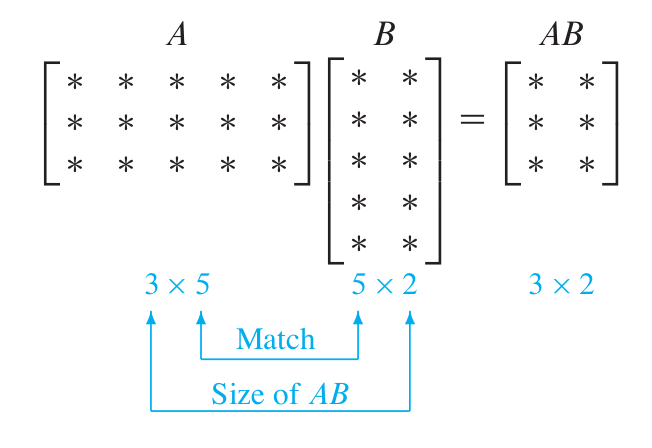
\includegraphics[width=\textwidth]{figures/Matrix_multiplication.png}
\end{column}
\end{columns}
}


\only<4>{
\textbf{4. Transpose of a Matrix}:
the transpose of a matrix is obtained by swapping its rows with its columns.

If \(A = [a_{ij}]\) is an \(m \times n\) matrix, then the transpose \(A^T = [a_{ji}]\) is an \(n \times m\) matrix.

\textbf{Example:}
\[
A = \begin{bmatrix} 1 & 2 \\ 3 & 4 \\ 5 & 6 \end{bmatrix}
\quad
\Rightarrow
\quad
A^T = \begin{bmatrix} 1 & 3 & 5 \\ 2 & 4 & 6 \end{bmatrix}.
\]

    \begin{center}\setlength{\fboxsep}{10pt}\fcolorbox{green!20}{green!20}{\parbox{0.9\linewidth}{
        \begin{theorem}
            Let \(A\) and \(B\) denote matrices whose sizes are appropriate for the following sums and products. The following is true:
            \begin{enumerate}[(i)]
                \item \((A^{\top})^{\top} = A\)
                \item \((A + B)^{\top} = A^{\top} + B^{\top}\)
                \item \((AB)^{\top} = B^{\top}A^{\top}\)
                \item \((rA)^{\top} = rA^{\top}\)
            \end{enumerate}
        \end{theorem}
    }}
    \end{center}

}


\only<5>{
\textbf{5. Determinant of a Square Matrix}:
the determinant is a scalar value that can be computed for square matrices.
\begin{center}\setlength{\fboxsep}{10pt}\fcolorbox{blue!20}{blue!20}{\parbox{0.9\linewidth}{
For a \(2 \times 2\) matrix \(A = \begin{bmatrix} a & b \\ c & d \end{bmatrix}\), the determinant is:
\[
\det(A) = ad - bc.
\]
}}
\end{center}

\textbf{Example:}
\[
A = \begin{bmatrix} 3 & 5 \\ 1 & 2 \end{bmatrix}.
\]
\[
\det(A) = (3)(2) - (5)(1) = 6 - 5 = 1.
\]
}


\only<6>{
\textbf{5. Determinant of a Square Matrix}

\begin{center}\setlength{\fboxsep}{10pt}\fcolorbox{blue!20}{blue!20}{\parbox{0.9\linewidth}{
For \(3 \times 3\) matrix) \(A = \begin{bmatrix} \mathcolor{red}{a} & \mathcolor{green}{b} & \mathcolor{blue}{c}\\ d & e & f\\ g & h & i \end{bmatrix}\) the determinant is:
\[
\det(A) = \mathcolor{red}{a} \cdot\det\left(\begin{bmatrix} e & f \\ h & i \end{bmatrix}\right)\; \mathbf{-} \; \mathcolor{green}{b}\cdot \det\left(\begin{bmatrix} d & f \\ g & i \end{bmatrix}\right)\; \mathbf{+} \; \mathcolor{blue}{c} \cdot \det\left(\begin{bmatrix} d & e \\ g & h \end{bmatrix}\right)\; .
\]
}}
\end{center}

}


\only<7>{
\textbf{6. Inverse of a Matrix}
The inverse of a square matrix \(A\) (if it exists) is a matrix \(A^{-1}\) such that:
\(
AA^{-1} = A^{-1}A = I,
\)
where \(I\) is the identity matrix.
\begin{center}\setlength{\fboxsep}{10pt}\fcolorbox{blue!20}{blue!20}{\parbox{0.9\linewidth}{
\textbf{Formula (for \(2 \times 2\) matrix):} If \(A = \begin{bmatrix} a & b \\ c & d \end{bmatrix}\) and \(\det(A) \neq 0\), then:
\[
A^{-1} = \frac{1}{\det(A)} \begin{bmatrix} d & -b \\ -c & a \end{bmatrix}.
\]
}}
\end{center}


\textbf{Example:}
\[
A = \begin{bmatrix} 2 & 1 \\ 3 & 4 \end{bmatrix}.
\]
\[
\det(A) = (2)(4) - (1)(3) = 8 - 3 = 5.
\]
\[
A^{-1} = \frac{1}{5} \begin{bmatrix} 4 & -1 \\ -3 & 2 \end{bmatrix} = \begin{bmatrix} 0.8 & -0.2 \\ -0.6 & 0.4 \end{bmatrix}.
\]
}


\only<8>{
\textbf{7. Identity Matrix}
The identity matrix \(I_n\) is a square matrix with ones on the diagonal and zeros elsewhere.
It acts as the multiplicative identity for matrices:
\[
AI = IA = A.
\]

\textbf{Example:}
\[
I_3 = \begin{bmatrix} 1 & 0 & 0 \\ 0 & 1 & 0 \\ 0 & 0 & 1 \end{bmatrix}.
\]
}
\end{frame}


\begin{frame}{Matrix Operations Summary}
\only<1>{
    \begin{center}\setlength{\fboxsep}{10pt}\fcolorbox{green!20}{green!20}{\parbox{0.9\linewidth}{
        \begin{theorem}
            Let \(A\) be an \(m\times n\) matrix, and let \(B\) and \(C\) have sizes for which the indicated sums and products are define:
            \begin{enumerate}[(i)]
                \item \textbf{Associativity:} \(A(BC)=(AB)C\)
                \item \textbf{Left Distribution:} \(A(B+C)=AC+BC\)
                \item \textbf{Right Distribution:} \((A+B)C=AC + BC\)
                \item \textbf{Scalar Distribution:} \(r(AB)=(rA)B=A(rB)\)
            \end{enumerate}
        \end{theorem}
    }}
    \end{center}

    \begin{center}\setlength{\fboxsep}{10pt}\fcolorbox{red!10}{red!10}{\parbox{0.9\linewidth}{
        \textbf{Note:} \(AB \neq BA\). 
            
        Also, there are no cancellation laws. That is, if \(AB=AC\), then it is not true in general that \(B=C\).
        }}
    \end{center}
}

\only<2>{
    \begin{center}\setlength{\fboxsep}{10pt}\fcolorbox{green!20}{green!20}{\parbox{0.9\linewidth}{
        \begin{theorem}
            If \(A\) and \(B\) are \(n\times n\) invertible matrices, then \(A^{-1}\) and \(B^{-1}\) are also invertible, and:
            \begin{enumerate}[(i)]
                \item  \((A^{-1})^{-1} = A\)
                \item \((AB)^{-1} = B^{-1}A^{-1}\)
                \item \textbf{Right Distribution:} \((A+B)C=AC + BC\)
                \item \((A^{-1})^{\top} = (A^{\top})^{-1}\), since \(A^{\top})\) is also invertible.
            \end{enumerate}
        \end{theorem}
    }}
    \end{center}
}
\end{frame}


\begin{frame}{Algorithm for Finding the Inverse of a Matrix Using Row Reductions}
\textbf{Algorithm Steps}
\begin{enumerate}
    \item Write the augmented matrix \([A \mid I_n]\).
    \item Use row operations to transform the left-hand side \(A\) into \(I_n\).
    \item Ensure all pivot elements (diagonal entries) are \(1\), and all other elements in the column are \(0\).
    \item Once the left-hand side is \(I_n\), the right-hand side will be \(A^{-1}\).
\end{enumerate}

\textbf{Conditions for Invertibility}
The matrix \(A\) is invertible if and only if:
\begin{enumerate}
    \item \(A\) is a square matrix.
    \item \(\det(A) \neq 0\) (i.e., \(A\) is full rank).
\end{enumerate}

\textbf{Important Notes}
\begin{itemize}
    \item If \(A\) cannot be row reduced to \(I_n\) (e.g., a row becomes zero during the process), \(A\) is not invertible.
    \item The algorithm is applicable only for square matrices.
\end{itemize}
\end{frame}



\begin{frame}{Examples}
\only<1>{
\begin{columns}
\begin{column}{0.5\textwidth}
\textbf{Example 1}
Let \(A = \begin{bmatrix} 2 & 1 \\ 1 & 1 \end{bmatrix}\). Find \(A^{-1}\).

\textbf{Solution:} Start with the augmented matrix:
\[[A \mid I_2] = 
\left[\begin{array}{cc|cc}
2 & 1 & 1 & 0 \\
1 & 1 & 0 & 1
\end{array}\right].
\]

Step 1: Scale the first row by \(\frac{1}{2}\):
\[
\left[\begin{array}{cc|cc}
1 & \frac{1}{2} & \frac{1}{2} & 0 \\
1 & 1 & 0 & 1
\end{array}\right].
\]

Step 2: Subtract the first row from the second row:
\[
\left[\begin{array}{cc|cc}
1 & \frac{1}{2} & \;\;\frac{1}{2} & 0 \\
0 & \frac{1}{2} & -\frac{1}{2} & 1
\end{array}\right].
\]
\end{column}

\begin{column}{0.5\textwidth}
Step 3: Scale the second row by \(2\):
\[
\left[\begin{array}{cc|cc}
1 & \frac{1}{2} & \;\;\frac{1}{2} & 0 \\
0 & 1 & -1 & 2
\end{array}\right].
\]

Step 4: Subtract \(\frac{1}{2}\) of the second row from the first row:
\[
\left[\begin{array}{cc|cc}
1 & 0 & \;\;1 & -1 \\
0 & 1 & -1 & \;\;2
\end{array}\right]
\]

Thus, \(A^{-1} = \begin{bmatrix} 1 & -1 \\ -1 & 2 \end{bmatrix}\).
\end{column}
\end{columns}
}


\only<2>{
\begin{columns}
\begin{column}{0.5\textwidth}
\textbf{Example 2}
Let \(A = \begin{bmatrix} 3 & 1 \\ 4 & 2 \end{bmatrix}\). Find \(A^{-1}\).

\textbf{Solution:} Start with the augmented matrix:
\[
\left[\begin{array}{cc|cc}
3 & 1 & 1 & 0 \\
4 & 2 & 0 & 1
\end{array}\right].
\]

Step 1: Scale the first row by \(\frac{1}{3}\):
\[
\left[\begin{array}{cc|cc}
1 & \frac{1}{3} & \frac{1}{3} & 0 \\
4 & 2 & 0 & 1
\end{array}\right].
\]

Step 2: Subtract 4 times the first row from the second row:
\[
\left[\begin{array}{cc|cc}
1 & \frac{1}{3} & \;\;\frac{1}{3} & 0 \\
0 & \frac{2}{3} & -\frac{4}{3} & 1
\end{array}\right].
\]
\end{column}

\begin{column}{0.5\textwidth}
Step 3: Scale the second row by \(\frac{3}{2}\):
\[
\left[\begin{array}{cc|cc}
1 & \frac{1}{3} & \;\;\frac{1}{3} & 0 \\
0 & 1 & -2 & \frac{3}{2}
\end{array}\right].
\]

Step 4: Subtract \(\frac{1}{3}\) of the second row from the first row:
\[
\left[\begin{array}{cc|cc}
1 & 0 & \;\;1 & -\frac{1}{2} \\
0 & 1 & -2 & \;\;\;\frac{3}{2}
\end{array}\right].
\]

Thus, \(A^{-1} = \begin{bmatrix} \;\;1 & -\frac{1}{2} \\ -2 & \;\;\;\frac{3}{2} \end{bmatrix}\).

\end{column}
\end{columns}
}

\only<3>{
\begin{columns}
\begin{column}{0.6\textwidth}
\textbf{Example 3:}
Find the inverse of \(A = \begin{bmatrix} 1 & 2 & 1 \\ 0 & 1 & 2 \\ 1 & 3 & 1 \end{bmatrix}.\)

\[
\left[\begin{array}{ccc|ccc}
1 & 2 & 1 & 1 & 0 & 0 \\
0 & 1 & 2 & 0 & 1 & 0 \\
1 & 3 & 1 & 0 & 0 & 1
\end{array}\right].
\]

Step 1: \(-R_1 + R_3 \to R_3\)
\[
\left[\begin{array}{ccc|ccc}
1 & 2 & 1 & 1 & 0 & 0 \\
0 & 1 & 2 & 0 & 1 & 0 \\
0 & 1 & 0 & -1 & 0 & 1
\end{array}\right].
\]
Step 2: Swap \(R_1\) and\( R_3\)
\[
\left[\begin{array}{ccc|ccc}
1 & 2 & 1 & 1 & 0 & 0 \\
0 & 1 & 0 & -1 & 0 & 1\\
0 & 1 & 2 & 0 & 1 & 0 
\end{array}\right].
\]
\end{column}

\begin{column}{0.5\textwidth}
Step 3: \(-R_2 +R_3 \to R_3\)
\[
\left[\begin{array}{ccc|ccc}
1 & 2 & 1 & 1 & 0 & 0 \\
0 & 1 & 0 & -1 & 0 & 1\\
0 & 0 & 2 & 1 & 1 & -1 
\end{array}\right].
\]

Step 3:  \(\frac{1}{2}R_3 \to R_3\):
\[
\left[\begin{array}{ccc|ccc}
1 & 2 & 1 & 1 & 0 & 0 \\
0 & 1 & 0 & -1 & 0 & 1\\
0 & 0 & 1 & \frac{1}{2} & \frac{1}{2} & -\frac{1}{2}
\end{array}\right].
\]

Continue until you obtain the inverse.

Thus, \(A^{-1} = \begin{bmatrix} \frac{5}{2} & -\frac{1}{2} & -\frac{3}{2} \\ -1 & 0 & 1 \\ \frac{1}{2} & \frac{1}{2} & -\frac{1}{2} \end{bmatrix}\).
\end{column}
\end{columns}
}

% \only<4>{
% \begin{columns}
% \begin{column}{0.5\textwidth}
% \textbf{Example 2:}
% Find the inverse of \[A = \begin{bmatrix} 2 & 1 & 3 \\ 1 & 1 & 1 \\ 3 & 2 & 4 \end{bmatrix}.\]
% \textbf{Solution:} Start with the augmented matrix:
% \[
% \left[\begin{array}{ccc|ccc}
% 2 & 1 & 3 & 1 & 0 & 0 \\
% 1 & 1 & 1 & 0 & 1 & 0 \\
% 3 & 2 & 4 & 0 & 0 & 1
% \end{array}\right].
% \]

% Step 1: Scale the first row by \(\frac{1}{2}\):
% \[
% \left[\begin{array}{ccc|ccc}
% 1 & \frac{1}{2} & \frac{3}{2} & \frac{1}{2} & 0 & 0 \\
% 1 & 1 & 1 & 0 & 1 & 0 \\
% 3 & 2 & 4 & 0 & 0 & 1
% \end{array}\right].
% \]
% \end{column}

% \begin{column}{0.5\textwidth}
% Step 2: Eliminate the first column in the second and third rows:
% \[
% \left[\begin{array}{ccc|ccc}
% 1 & \frac{1}{2} & \frac{3}{2} & \frac{1}{2} & 0 & 0 \\
% 0 & \frac{1}{2} & -\frac{1}{2} & -\frac{1}{2} & 1 & 0 \\
% 0 & \frac{1}{2} & -\frac{1}{2} & -\frac{3}{2} & 0 & 1
% \end{array}\right].
% \]

% Step 3: Scale the second row by 2:
% \[
% \left[\begin{array}{ccc|ccc}
% 1 & \frac{1}{2} & \frac{3}{2} & \frac{1}{2} & 0 & 0 \\
% 0 & 1 & -1 & -1 & 2 & 0 \\
% 0 & \frac{1}{2} & -\frac{1}{2} & -\frac{3}{2} & 0 & 1
% \end{array}\right].
% \]

% Continue reducing until:
% \[
% A^{-1} = \begin{bmatrix}
% 1 & -1 & 0 \\
% -3 & 4 & -1 \\
% 2 & -2 & 1
% \end{bmatrix}.
% \]
% \end{column}
% \end{columns}
% }
\end{frame}


\begin{frame}{Homework 6}
\begin{enumerate}
    \item Find the inverse of \(A = \begin{bmatrix} 2 & 3 \\ 1 & 4 \end{bmatrix}\) if it exists.
    \item Determine whether \(A = \begin{bmatrix} 1 & 2 \\ 2 & 4 \end{bmatrix}\) is invertible. Justify your response.
    \item Verify that the inverse you found for \(A = \begin{bmatrix} 2 & 1 \\ 1 & 1 \end{bmatrix}\) satisfies \(AA^{-1} = I\).
    \item Find the inverse of \(A = \begin{bmatrix} 1 & 2 & 3 \\ 0 & 1 & 4 \\ 5 & 6 & 0 \end{bmatrix}\).
    \item Verify that the matrix \(A = \begin{bmatrix} 2 & 1 & 0 \\ -1 & 1 & 2 \\ 3 & -2 & 1 \end{bmatrix}\) is invertible and find its inverse.
    \item Show that the matrix \(A = \begin{bmatrix} 1 & 2 & 3 \\ 4 & 5 & 6 \\ 7 & 8 & 9 \end{bmatrix}\) is not invertible.
\end{enumerate}

\end{frame}

\subsection{Characterization of Invertible Matrices}
\begin{frame}{Characterization of Invertible Matrices}
\begin{center}\setlength{\fboxsep}{10pt}\fcolorbox{green!20}{green!20}{\parbox{0.9\linewidth}{
        \begin{theorem}[Invertible Matrix Theorem]
            Let \(A\) be an \(n\times n\) matrix.
            Then the following statements are equivalent.
            That is, for a given $A$, the statements are either \textcolor{blue}{\textbf{all TRUE}} or \textcolor{red}{\textbf{all FALSE}}.
            \begin{enumerate}[(a)]
                \item  \(A\) is an invertible matrix. \(A^{\top}\) is also invertible.
                \item  \(A\) is row equivalent to an \(n\times n\) identity matrix.
                \item \(A\) has a pivot in each row after row reduction.
                \item The matrix equation, \(A\mathbf{x}=\mathbf{b}\) has a solution for each \(\mathbf{b} \in \mathbb{R}^n\).
                \item The columns of \(A\) span \(\mathbb{R}^n\).
                \item The columns of \(A\) are linearly independent.
                \item The homogeneous equation, \(A\mathbf{x}=\mathbf{0}\) has only the trivial solution.
                \item The linear transformation \(T(\mathbf{x}) = A\mathbf{x}\) is one-to-one
                \item The linear transformation \(T(\mathbf{x}) = A\mathbf{x}\) is onto.
            \end{enumerate}
        \end{theorem}
    }}
    \end{center}
\end{frame}


\begin{frame}{Characterization of Invertible Matrices}
\begin{center}\setlength{\fboxsep}{10pt}\fcolorbox{green!20}{green!20}{\parbox{0.9\linewidth}{
        \begin{theorem}
            Let \(T:\mathbb{R}^n \to \mathbb{R}^n\) be a linear transformation such that \(T(\mathbf{x})=A\mathbf{x}\), where \(A\) is the transformation matrix.
            Then \(T\) is invertible if and only if \(A\) is an invertible matrix.

            And the inverse of the transformation \(T^{-1}:\mathbb{R}^n \to \mathbb{R}^n\) is \(T^{-1}(\mathbf{x}) = A^{-1}\mathbf{x}\)
        \end{theorem}
    }}
    \end{center}
\end{frame}


\begin{frame}{Homework 7}
\begin{enumerate}
    % \item If \(A\) is invertible, then the columns of \(A^{-1}\) are linearly independent. True or false? Explain your answer.
    \item Is \(A = \begin{bmatrix}
        0 & \;\;\;2 & -2 & 3\\
        0 & \;\;\;0 & \;\;0 & 5\\
        1 & -4 & \;\; 8 & 1
    \end{bmatrix}\) one-to-one? Explain the reason for your answer.
    \item Let \( T: \mathbb{R}^2 \to \mathbb{R}^2 \) be a linear transformation defined by:
    \(
    T\left(\left[\begin{array}{c} x \\y \end{array}\right]\right) = 
    \left[\begin{array}{c} 2x + 3y\\ x + 4y \end{array}\right].
    \)
    Write out \(T\) in the form, \(T(\mathbf{x}) = A\mathbf{x}.\)
    
    Is \(T\) is invertible? If so, find a formula for \(T^{-1}.\)
\end{enumerate}
\end{frame}

\subsection{Subspaces of \(\mathbb{R}^2\)}
\begin{frame}{Subspaces of \(\mathbb{R}^n\)}
\only<1>{
    \begin{center}\setlength{\fboxsep}{10pt}\fcolorbox{blue!20}{blue!20}{\parbox{0.9\linewidth}{
        \begin{definition}
            A \textbf{subspace} of \(\mathbb{R}^n\) is any set \(S \in \mathbb{R}^n\) that has 3 properties:
            \begin{enumerate}[i)]
                \item The zero vector is in \(S\).
                \item For each \(\mathbf{u},\; \mathbf{v} \in S\), \(\mathbf{u}+\mathbf{v}\in S\).
                \item For each \(\mathbf{u} \in S\), and scalar \(c\in\mathbb{R}\),  \(c\mathbf{u}\in S\).
            \end{enumerate}
        \end{definition}
    }}
    \end{center}

\textbf{Example:} If \(\mathbf{u}_1,\; \mathbf{u}_2 \in \mathbb{R}^n\), and \(S=Span(\{\mathbf{u}_1,\; \mathbf{u}_2\})\).
Then \(S\) is a subspace of \(\mathbb{R}^n\).
}


\only<2>{
    \begin{center}\setlength{\fboxsep}{10pt}\fcolorbox{blue!20}{blue!20}{\parbox{0.9\linewidth}{
        \begin{definition}
            A \textbf{column space} of matrix \(A\) is the set, \(Col A = Span(\{\text{Columns of } A\})\).  That is, the set of all linear combinations of the columns of \(A\).
        \end{definition}
    }}
    \end{center}

\textbf{Example:} Let 
    \(A = \begin{bmatrix}
        \;\;\;1 & -3 & -4\\
        -4 & \;\;\; 6 & -2\\
        -3 & \;\;\; 7 & \;\;\;6
    \end{bmatrix}\)
    and
    \(\mathbf{b} = \begin{bmatrix}
        \;\;\;5\\
        \;\;\;3\\
        -4
    \end{bmatrix}\).
    Determine whether \(\mathbf{b}\) is in the column space of \(A\).
}


\only<3>{
    \begin{center}\setlength{\fboxsep}{10pt}\fcolorbox{blue!20}{blue!20}{\parbox{0.9\linewidth}{
        \begin{definition}
        A \textbf{null space} of matrix \(A\) is the set, \(Nul A\) - of all solutions of the homogeneous equation \(A\mathbf{x}=\mathbf{0}\).
        \end{definition}
    }}
    \end{center}

\begin{center}\setlength{\fboxsep}{10pt}\fcolorbox{green!20}{green!20}{\parbox{0.9\linewidth}{
        \begin{theorem}
        A \textbf{null space} of and \(m\times n\) matrix \(A\) is a subspace of \(\mathbb{R}^n\). Equivalently, the set of all solutions of the homogeneous system \(A\mathbf{x}=\mathbf{0}\) is also a subspace of \(\mathbb{R}^n\).
        \end{theorem}
    }}
    \end{center}
}

\end{frame}


\begin{frame}{Basis}
    \begin{center}\setlength{\fboxsep}{10pt}\fcolorbox{blue!20}{blue!20}{\parbox{0.9\linewidth}{
        \begin{definition}
        A \textbf{basis} of a subspace \(S\) of \(\mathbb{R}^n\) is a linearly independent set in \(S\) that spans \(S\).
        \end{definition}

        \textbf{Note:} The number of pivots tells you the number of basis elements the \textbf{null space} and \textbf{column space}.

        \[
        \text{\# of basis elements in null space} \mathbf{+} \text{\# of basis elements in column space} = \text{\# of columns}
        \]
    }}
    \end{center}

\only<1>{
\begin{center}\setlength{\fboxsep}{10pt}\fcolorbox{green!20}{green!20}{\parbox{0.9\linewidth}{
        \begin{theorem}
        A \textbf{pivot columns} of a matrix \(A\) form a basis for the columns space of \(A\).
        \end{theorem}
    }}
    \end{center}
}


\only<2>{
\textbf{Example 1:} Find the basis for the null space, and the basis of the column space of the matrix
\[
    A = \begin{bmatrix}
        -3 & \;\;\;6 & -1 & 1 & -7\\
        \;\;\;1 & -2 & \;\;\;2 & 3 & -1\\
        \;\;\;2 & -4 & \;\;\;5 & 8 & -4
    \end{bmatrix}
    \]
}

\only<3>{
\textbf{Example 2:} Find the basis for the null space, and the basis of the column space of the matrix
\[
    A = \begin{bmatrix}
        1 & 0 & -3 & \;\;\;5 & 0\\
        0 & 1 & \;\;\;2 & -1 & 0\\
        0 & 0 & \;\;\;0 & \;\;\;0 & 1\\
         0 & 0 & \;\;\;0 & \;\;\;0 & 0
    \end{bmatrix}
    \]
}
\end{frame}


\begin{frame}{Homework 8}
\textbf{Question 1:} Find the basis for the null space, and the basis of the column space of the matrix
\[
    A = \begin{bmatrix}
        \;\;\;1 & \;\;\;3 & \;\;\;3 & \;\;\;2 & -9\\
        -2 & -2 & \;\;\;2 & -8 & \;\;\;2\\
        \;\;\;2 & \;\;\;3 & \;\;\;0 & \;\;\;7 & \;\;\;1\\
         \;\;\;3 & \;\;\;4 & -1 & \;\;\;11 & -8
    \end{bmatrix}
    \]
\end{frame}

\subsection{Dimension and Rank}
\begin{frame}{Dimension of a Subspace}
    \begin{center}\setlength{\fboxsep}{10pt}\fcolorbox{blue!20}{blue!20}{\parbox{0.9\linewidth}{
        \begin{definition}
        The \textbf{dimension} of a nonzero subspace \(S\), denoted by dim\(S\) is the number of vectors in a basis for the subspace \(S\).
        
        The dimension of the zero subspace \(\{\mathbf{0}\}\) is defined to be zero.
        \end{definition}
    }}
    \end{center}


    \begin{center}\setlength{\fboxsep}{10pt}\fcolorbox{blue!20}{blue!20}{\parbox{0.9\linewidth}{
        \begin{definition}
        The \textbf{rank} of a matrix \(A\), denoted by rank\(A\) is the dimension of the column space of \(A\).
        
        The dimension of the zero subspace \(\{\mathbf{0}\}\) is defined to be zero.
        \end{definition}
    }}
    \end{center}

    \begin{center}\setlength{\fboxsep}{10pt}\fcolorbox{green!20}{green!20}{\parbox{0.9\linewidth}{
        \begin{theorem}[Rank Theorem]
        If a matrix \(A\) has \(n\) columns, then rank\(A\) + dim(Nul\(A\)).
        \end{theorem}
    }}
    \end{center}
\end{frame}

\begin{frame}{Examples}

\textbf{Example 1:} Determine the rank and dim(Nul\(A\)) of the matrix below
\[
    A = \begin{bmatrix}
        -3 & \;\;\;6 & -1 & 1 & -7\\
        \;\;\;1 & -2 & \;\;\;2 & 3 & -1\\
        \;\;\;2 & -4 & \;\;\;5 & 8 & -4
    \end{bmatrix}
    \]

\textbf{Example 2:} etermine the rank and dim(Nul\(A\)) of the matrix below
\[
    B = \begin{bmatrix}
        1 & 0 & -3 & \;\;\;5 & 0\\
        0 & 1 & \;\;\;2 & -1 & 0\\
        0 & 0 & \;\;\;0 & \;\;\;0 & 1\\
         0 & 0 & \;\;\;0 & \;\;\;0 & 0
    \end{bmatrix}
    \]
    
\end{frame}



\begin{frame}{Characterization of Invertible Matrices Cont'd}
\begin{center}\setlength{\fboxsep}{10pt}\fcolorbox{green!20}{green!20}{\parbox{0.9\linewidth}{
        \begin{theorem}[Invertible Matrix Theorem Continued]
            Let \(A\) be an \(n\times n\) matrix.
            Then the following statements are equivalent.
            That is, for a given $A$, the statements are either \textcolor{blue}{\textbf{all TRUE}} or \textcolor{red}{\textbf{all FALSE}}.
            \begin{enumerate}
                \item[(a)] \(A\) is an invertible matrix. \(A^{\top}\) is also invertible.
                \item[(c)] \(A\) has a pivot in each row after row reduction.
                \item[(j)] Let \(A\) be and \(n\times n\) matrix .
                \item[(k)] The columns of \(A\) form a basis of \(\mathbb{R}^n\).
                \item[(l)] The column space of \(A\), Col\(A\)=\(\mathbb{R}^n\).
                \item[(m)] The dimension of the column space of \(A\), dim Col\(A\) = \(n\).
                \item[(n)] rank\(A\) = \(n\).
                \item[(o)] The null space of \(A\), Nul\(A\) = \(\{\mathbf{0}\}\).
                \item[(p)] The dimension of the null space of \(A\), dim Nul\(A\) = \(0\).
            \end{enumerate}
        \end{theorem}
    }}
    \end{center}
\end{frame}


\section{Determinants}
\subsection{Introduction to Determinants}

\begin{frame}{Introduction to Determinants}
\only<1>{
\textbf{Intuition:}
Geometrically, the \textcolor{blue}{determinant  of a matrix \(A\) measures the scaling factor} after applying the matrix transformation \(T(\mathbf{x}) = A\mathbf{x}\) .

In a  $2 \times 2$ matrix, the scaling factor measures how much bigger/smaller the area of the unit square gets after the transformation has been applied. For  a $3 \times 3$ matrix, how much bigger volume of the unit cube gets after the transformation has been applied.

If $\det(A) = 0$, the transformation collapses space into a lower dimension, implying that $A$ is non-invertible (singular/ does not have an inverse).

For example:
\begin{itemize}
    \item If a $2 \times 2$ matrix has a determinant of 5, it scales areas by a factor of 5.
    \item If a $3 \times 3$ matrix has a determinant of -2, it scales volumes by a factor of 2 and reverses orientation (flips it like a page).
\end{itemize}
}

\only<2>{
\begin{center}\setlength{\fboxsep}{10pt}\fcolorbox{blue!20}{blue!20}{\parbox{0.9\linewidth}{
\begin{definition}[Determinant]
The determinant of a square matrix $A$ of order $n \times n$ is a scalar value that provides important information about the matrix, such as whether it is invertible and how it scales volumes in linear transformations. The determinant of a matrix $A$ is denoted as $\det(A)$ or $|A|$.

For a $2 \times 2$ matrix:
\begin{equation*}
    A = \begin{bmatrix} a & b \\ c & d \end{bmatrix},\;\;
    \text{its determinant is given by: }\;
    \det(A) = ad - bc.
\end{equation*}

For a $3 \times 3$ matrix:
\begin{equation*}
    A = \begin{bmatrix} a & b & c \\ d & e & f \\ g & h & i \end{bmatrix},\;\;\;
    \det(A) = a \begin{vmatrix} e & f \\ h & i \end{vmatrix} - b \begin{vmatrix} d & f \\ g & i \end{vmatrix} + c \begin{vmatrix} d & e \\ g & h \end{vmatrix}.
\end{equation*}

\end{definition}
}}
\end{center}
}

\only<3>{
\textbf{Example 1}

Given the matrix:
\begin{equation*}
    A = \begin{bmatrix} 3 & 2 \\ 1 & 4 \end{bmatrix},
\end{equation*}
its determinant is:
\begin{equation*}
    \det(A) = (3)(4) - (2)(1) = 12 - 2 = 10.
\end{equation*}

\textbf{Example 2}

Consider the matrix:
\begin{equation*}
    B = \begin{bmatrix} 1 & 2 \\ 2 & 4 \end{bmatrix},
\end{equation*}
its determinant is:
\begin{equation*}
    \det(B) = (1)(4) - (2)(2) = 4 - 4 = 0.
\end{equation*}
Since the determinant is zero, $B$ is singular and non-invertible.
}

\only<4>{
\begin{center}\setlength{\fboxsep}{9pt}\fcolorbox{blue!20}{blue!20}{\parbox{0.9\linewidth}{
\begin{definition}[Generalized Definition of Determinant]
The \textbf{determinant} of a square matrix $A=[a_{ij}]$ of order $n \times n$ is the sum of \(n\) terms of the form \(\pm a \det(A_{ij})\), with plus and minus signs alternating, where the entries \(a_{11}, a_{12},\ldots,a_{1n}\) are from the first row of\(A\) \textcolor{red}{(not entirely true)}.
\textbf{Matrix} \(A_{ij}\) \textbf{is obtained by deleting the} \(i\)\textbf{th row and the} \(j\)\textbf{th column}.
\begin{align*}
    \det(A) \text{ or } |A| =& \sum_{j=1}^n (-1)^{1+j}a_{1j}\det(A_{1j})\\
    =& a_{11}\det(A_{11})- a_{12}\det(A_{12})+a_{13}\det(A_{13})- \cdots +(-1)^{1+n}a_{1n}\det(A_{1n})
\end{align*}
\end{definition}
}}
\end{center}

\textbf{Example:} Compute the determinant of 
\(
 A = \begin{bmatrix} 2 & 4 & -1 \\ 0 & -2 & 0 \\ 1 & 5 & 0 \end{bmatrix}\;\;\;
 \)
}


\only<5>{
\begin{center}\setlength{\fboxsep}{10pt}\fcolorbox{blue!20}{blue!20}{\parbox{0.9\linewidth}{
\begin{definition}[Cofactor Definition of Determinant]
The \textbf{cofactor} of a matrix \(A\) is the number \(C_{ij}\) given by
\(
C_{ij} = (-1)^{i+j}\det(A_{ij}).
\)

The \textbf{determinant} of a square matrix $A=[a_{ij}]$ of order $n \times n$ can be computed using a \textbf{cofactor expansion} across the first row of\(A\) \textcolor{red}{(not entirely true)}.
\begin{align*}
    \det(A) \text{ or } |A|
    = a_{11}C_{11} + a_{12}C_{12}+a_{13}C_{13} + \cdots + a_{1n}C_{1n}
\end{align*}

\end{definition}
}}
\end{center}

\textbf{Example:} Compute the determinants of 
\(
 A = \begin{bmatrix} 2 & 4 & -1 \\ 0 & -2 & 0 \\ 1 & 5 & 0 \end{bmatrix},\;\;\;\text{and }\;
 B = \begin{bmatrix} 2 & -7 & 8 & 9 & -6 \\
                     0 &  2 & -5 & 7 & 3 \\
                     0 & 0 & 1 & 5 & 0 \\
                     0 & 0 & 2 & 4 & -1 \\
                     0 & 0 & 0 & -2 & 0\end{bmatrix}
 \)
}

\only<6>{
\textbf{Recall:} when we row reduce a matrix, it does not change the matrix.

Hence this can make the computation of the determinant easier!
    \begin{center}\setlength{\fboxsep}{10pt}\fcolorbox{green!20}{green!20}{\parbox{0.9\linewidth}{
        \begin{theorem}[Determinant Theorem]
        If \(A\) \textbf{is a triangular matrix}, then \(\det A\) is a product of the entries on the main diagonal of \(A\)).
        \end{theorem}
    }}
    \end{center}

    \begin{center}\setlength{\fboxsep}{10pt}\fcolorbox{green!20}{green!20}{\parbox{0.9\linewidth}{
        \begin{theorem}[Row Operations]
        Let \(A\) a square matrix.
        \begin{enumerate}[(a)]
            \item If a multiple of one row of \(A\) is added to another row to produce a matrix \(B\), then \(\det A = \det B\).
            \item If two rows of \(A\) are interchanged to produce a matrix \(B\), then \(\det A = -\det B\).
            \item If a row of \(A\) is multiplied by \(k\) to produce a matrix \(B\), then \(\det B = k \cdot\det A\).
        \end{enumerate}
        \end{theorem}
    }}
    \end{center}
}
\end{frame}


\subsection{Properties of Determinants}
\begin{frame}{Properties of Determinants}
    \begin{center}\setlength{\fboxsep}{10pt}\fcolorbox{green!20}{green!20}{\parbox{0.97\linewidth}{
    \begin{theorem}[Properties of Determinants]
    \begin{enumerate}[(a)]
    \only<1>{
        \item \textbf{Determinant of Identity:} The determinant of the identity matrix $I_n$ is 1, i.e., $\det(I_n) = 1$.
        
        \item \textbf{Row or Column Swap:} Swapping two rows or columns of a matrix $A$ to produce $B$ negates its determinant:
        \begin{equation*}
            \det(B) = -\det(A),
        \end{equation*}
        
        \item \textbf{Multiplication by a Scalar:} Multiplying a row or a column by a scalar $k$ multiplies the determinant by $k$:
        Therefore multiplying all \(n\) rows of a matrix by \(k\),
        \begin{equation*}
            \det(kA) = k^n \det(A).
        \end{equation*}
        
        \item \textbf{Triangular Matrices:} The determinant of a triangular (upper or lower) matrix is the product of its diagonal elements:
        \begin{equation*}
            \det(A) = a_{11} a_{22} \dots a_{nn}.
        \end{equation*}
    }
    \only<2>{
        \item[(e)] \textbf{Determinant of a Product:} The determinant of the product of two matrices is the product of their determinants:
        \begin{equation*}
            \det(AB) = \det(A)\cdot \det(B).
        \end{equation*}
        
        \item[(f)] \textbf{Effect of Row Operations:} Adding a multiple of one row to another does not change the determinant.
        \item[(g)] \textbf{Invertibility:} A square matrix $A$ is invertible if and only if $\det(A) \neq 0$.
        \item[(h)] \textbf{Transpose Property:} The determinant of a matrix is equal to the determinant of its transpose:
        \begin{equation*}
            \det(A^T) = \det(A).
        \end{equation*}
    }
    \end{enumerate}
    \end{theorem}
    }}
    \end{center}
\end{frame}



\subsection{Cramer's Rule, Volume, and Linear Transformations}
\begin{frame}{Cramer's Rule, Volume, and Linear Transformations}
\only<1>{
\textbf{Cramer's Rule}    
Cramer's rule is needed in a variety of theoretical calculations.
It can be used to study how the solution of \(A\mathbf{x}=\mathbf{b}\) is affected by changes in the entries of \(\mathbf{b}\).
However, the formula is inefficient for hand calculations, except for \(2 \times 2\) or \(3\times 3\) matrices.

Cramer's Rule provides an explicit formula for solving a system of linear equations using determinants.
Given a system of $n$ linear equations in $n$ variables represented in matrix form as:
\begin{equation*}
    A\mathbf{x} = \mathbf{b},
\end{equation*}
where $A$ is an $n \times n$ invertible matrix, the solution for each variable $x_i$ is given by:
\begin{equation*}
    x_i = \frac{\det(A_i)}{\det(A)},
\end{equation*}
\textbf{where} $A_i$ \textbf{is the matrix obtained by replacing the} $i$\textbf{-th column of} $A$ \textbf{with the column vector} $\mathbf{b}$.
}

\only<2>{
\textbf{Example 1:}
Consider the system,
\begin{align*}
    2x_1 + 3x_2 &= 5, \\
    4x_1 + x_2 &= 6.
\end{align*}
The coefficient matrix is:
\begin{equation*}
    A = \begin{bmatrix} 2 & 3 \\ 4 & 1 \end{bmatrix},
\end{equation*}
with determinant:
\begin{equation*}
    \det(A) = (2)(1) - (3)(4) = 2 - 12 = -10.
\end{equation*}
Replacing the first column with $\mathbf{b} = \begin{bmatrix} 5 \\ 6 \end{bmatrix} \; \text{ gives } \;
    A_1 = \begin{bmatrix} 5 & 3 \\ 6 & 1 \end{bmatrix},
$
with $\det(A_1) = (5)(1) - (3)(6) = 5 - 18 = -13$. Thus,
\begin{equation*}
    x_1 = \frac{\det(A_1)}{\det(A)} = \frac{-13}{-10} = 1.3.
\end{equation*}
Repeating for $A_2$ yields $x_2 = 0.8$.
}


\only<3>{
\begin{center}\setlength{\fboxsep}{10pt}\fcolorbox{blue!20}{blue!20}{\parbox{0.9\linewidth}{
\begin{definition}[Cofactor Formula for Inverse \(A^{-1}\)]
Let \(A\) be an invertible \(n\times n\) matrix. Then
\begin{eqnarray*}
A^{-1} =& \frac{1}{\det A}\cdot \text{adj}\,A\\
=& \frac{1}{\det A}\cdot
\begin{bmatrix}
    C_{11} & C_{12} & \cdots & C_{1n}\\
    C_{21} & C_{22} & \cdots & C_{2n}\\
    \vdots & \vdots & \ddots & \vdots\\
    C_{n1} & C_{n2} & \cdots & C_{nn}\\
\end{bmatrix}
\end{eqnarray*}

\(
C_{ij} = (-1)^{i+j}\det(A_{ij}).
\) \textbf{Matrix} \(A_{ij}\) \textbf{is obtained by deleting the} \(i\)\textbf{th row and the} \(j\)\textbf{th column}.

\end{definition}
}}
\end{center}
}


\only<4>{
\begin{center}\setlength{\fboxsep}{10pt}\fcolorbox{green!20}{green!20}{\parbox{0.9\linewidth}{
\begin{theorem}[Determinant-Area]
If \(A\) is a \(2\times 2\) matrix, 
\[\text{the area of the parallelogram determined by the columns of }A = |\det A|.\]
\end{theorem}
}}
\end{center}

}


\only<5>{
\begin{center}\setlength{\fboxsep}{10pt}\fcolorbox{green!20}{green!20}{\parbox{0.9\linewidth}{
\begin{theorem}[Determinant-Area]
Let \(T:\mathbb{R}^2 \to \mathbb{R}^2\) be a linear transformation determined by \(2\times 2\) matrix \(A\). 
If \(S\) is a parallelogram in \(\mathbb{R}^2\), then
\[\{\text{area of }T(S)\} = |\det A|\cdot \{\text{area of }S\}.\]
\end{theorem}
}}
\end{center}

\textbf{Example:}

Let \(S\) be the parallelogram determined by \(\mathbf{b}_1=\begin{bmatrix}
    1\\3
\end{bmatrix}\)
and 
\(\mathbf{b}_2=\begin{bmatrix}
    5\\1
\end{bmatrix}\),
and let 
\(A = \begin{bmatrix}
    1 & -1 \\ 0 & 2
\end{bmatrix}\).

Compute the area of the image of \(S\) under the mapping \(\mathbf{x} \rightarrow A\mathbf{x}\).
}
\end{frame}





%===================================================================================================================================================

\section*{Selected References}
\begin{frame}[allowframebreaks]
\printbibliography
\end{frame}

\end{document}
